\documentclass{article}
\usepackage{hypernat}              % ensure cooperation of natbib and hyperref
\usepackage{booktabs}
\usepackage[below]{placeins}
\usepackage{fancyhdr}
\usepackage{mdwlist}
\usepackage{indentfirst}
\usepackage[Symbol]{upgreek}
\usepackage{bm}
\usepackage{framed}
\usepackage{threeparttable}
\usepackage{overpic}
\usepackage{booktabs}
\usepackage{ctex}

\graphicspath{{F:/Cloud/GitHub/tgmf/figs/}{F:/Cloud/GitHub/doctor/figs/}{F:/Cloud/GitHub/doctor/figs/python/}{F:/Cloud/GitHub/doctor/figs/ppt/}{F:/Cloud/GitHub/doctor/figs/svg/}{F:/Cloud/GitHub/doctor/figs/sem/}{F:/Cloud/GitHub/doctor/figs/test/}}

\begin{document}
\title{镍基高温合金热梯度机械疲劳条件下的寿命预测}

\author{袁荒,孙经雨}
\date{\today}
\maketitle
\tableofcontents

\section*{摘要}
对于燃气轮机,内部冷却是降低零件温度,保证零件正常运转的重要手段。
设计和开展中心冷却的镍基高温合金热梯度机械疲劳(TGMF)试验。
与无温度梯度的热机械疲劳(TMF)寿命相比,TGMF的寿命要明显降低。
考虑温度与机械载荷相位对TGMF寿命的影响,在低周疲劳的情况下,TGMF同相位(IP)的寿命要明显低于反相位(OP)的寿命。
同时研究涂覆热障涂层(TBC)对镍基高温合金的热梯度机械疲劳性能的影响,结果表明,涂覆有热障涂层的试样寿命高于无涂层的试样寿命,但仍低于TMF试样寿命。
温度梯度会导致应力场的变化,通过有限元计算,确定试件在每个循环内的温度场分布,同时基于循环塑性本构方程计算当前温度场下的应力应变曲线。
选取多种多轴疲劳模型对试验数据进行预测,误差较大,引入温度梯度的修正项,建立热梯度机械疲劳寿命预测模型。

\section{概述}
热障涂层涂覆于航空发动机和燃气轮机高温部件表面,具有防止高温腐蚀、延长热端部件使用寿命、提高发动机功率和减少燃油消耗等优点。
通常典型的热障涂层包括表面陶瓷层(TC:top coat)和金属粘结层(BC:bond coat)。在服役过程中,粘结层会发生氧化,在粘结层和陶瓷层界面形成厚度为1~10$\mu$m的热生长氧化物(TGO:thermally grown oxide)。TGO的形成是一个体积膨胀过程,界面会限制这种体积变化,因而在TGO内部会随之产生应力。而且,陶瓷层与金属基底的热膨胀系数相
差较大,在热循环过程中会在热载荷的作用下产生较大的热应力,从而在界面缺陷处引起应力集中,促进裂纹的萌生与扩展。
\section{试验}

发动机涡轮叶片主要采用气膜冷却和内部流冷却,轮盘通常采用内部二次流冷却。
服役过程中,涡轮叶片不仅受到较大的交变载荷,而且在叶片表面和内部分别受到高温高压燃气的冲击和冷却气体的作用,这样涡轮叶片就遭受载荷和温度同时变化带来的热机械疲劳损伤。
此外,为了增强发动机冷却效果,提高发动机效率,先进的航空发动机和燃气轮机热端涡轮叶片多为薄壁多孔结构。
因此,我们设计了薄壁圆管试件来模拟零件的冷却结构,同时试件外壁涂覆有热障涂层。
在内部冷却气体作用下,试件内表面与外表面之间会产生很大的温度梯度,同时导致额外的应力,在热表面上表现为多轴压缩载荷,而在冷却表面上表现为多轴拉伸载荷。

对于薄壁圆管试件,我们可选择的加热方式有电阻炉、电磁感应、火焰喷射和辐射。
电阻炉的优点在于温度稳定性好,但实际发动机启动阶段升温过程只需要几十秒钟的时间,而且降温也相当迅速,采用电阻炉无法实现试件的快速升温和降温。
电磁感应加热的优点在于加热效率高,试件升温迅速,通常热机械疲劳试验采用高频电磁感应设备进行加热,其中高频电磁感应加热厚度约为1-2mm,这意味着试件的内外表面是同时加热的,在内部冷却过程中,不利于产生内外表面的温度梯度,同时电磁感应方式只会对内部金属层加热,使得内部金属层温度高于外部陶瓷层温度,这不符合热障涂层构件实际工作状态下的温度分布\cite{BRENDEL2008234}。
火焰喷射的优点在于接近真实发动机涡轮叶片的工作环境,但火焰的稳定性差,火焰形状难以控制,很难形成均匀的温度场\cite{MAUGET2017225}。

\begin{figure}[!htp]
\centering{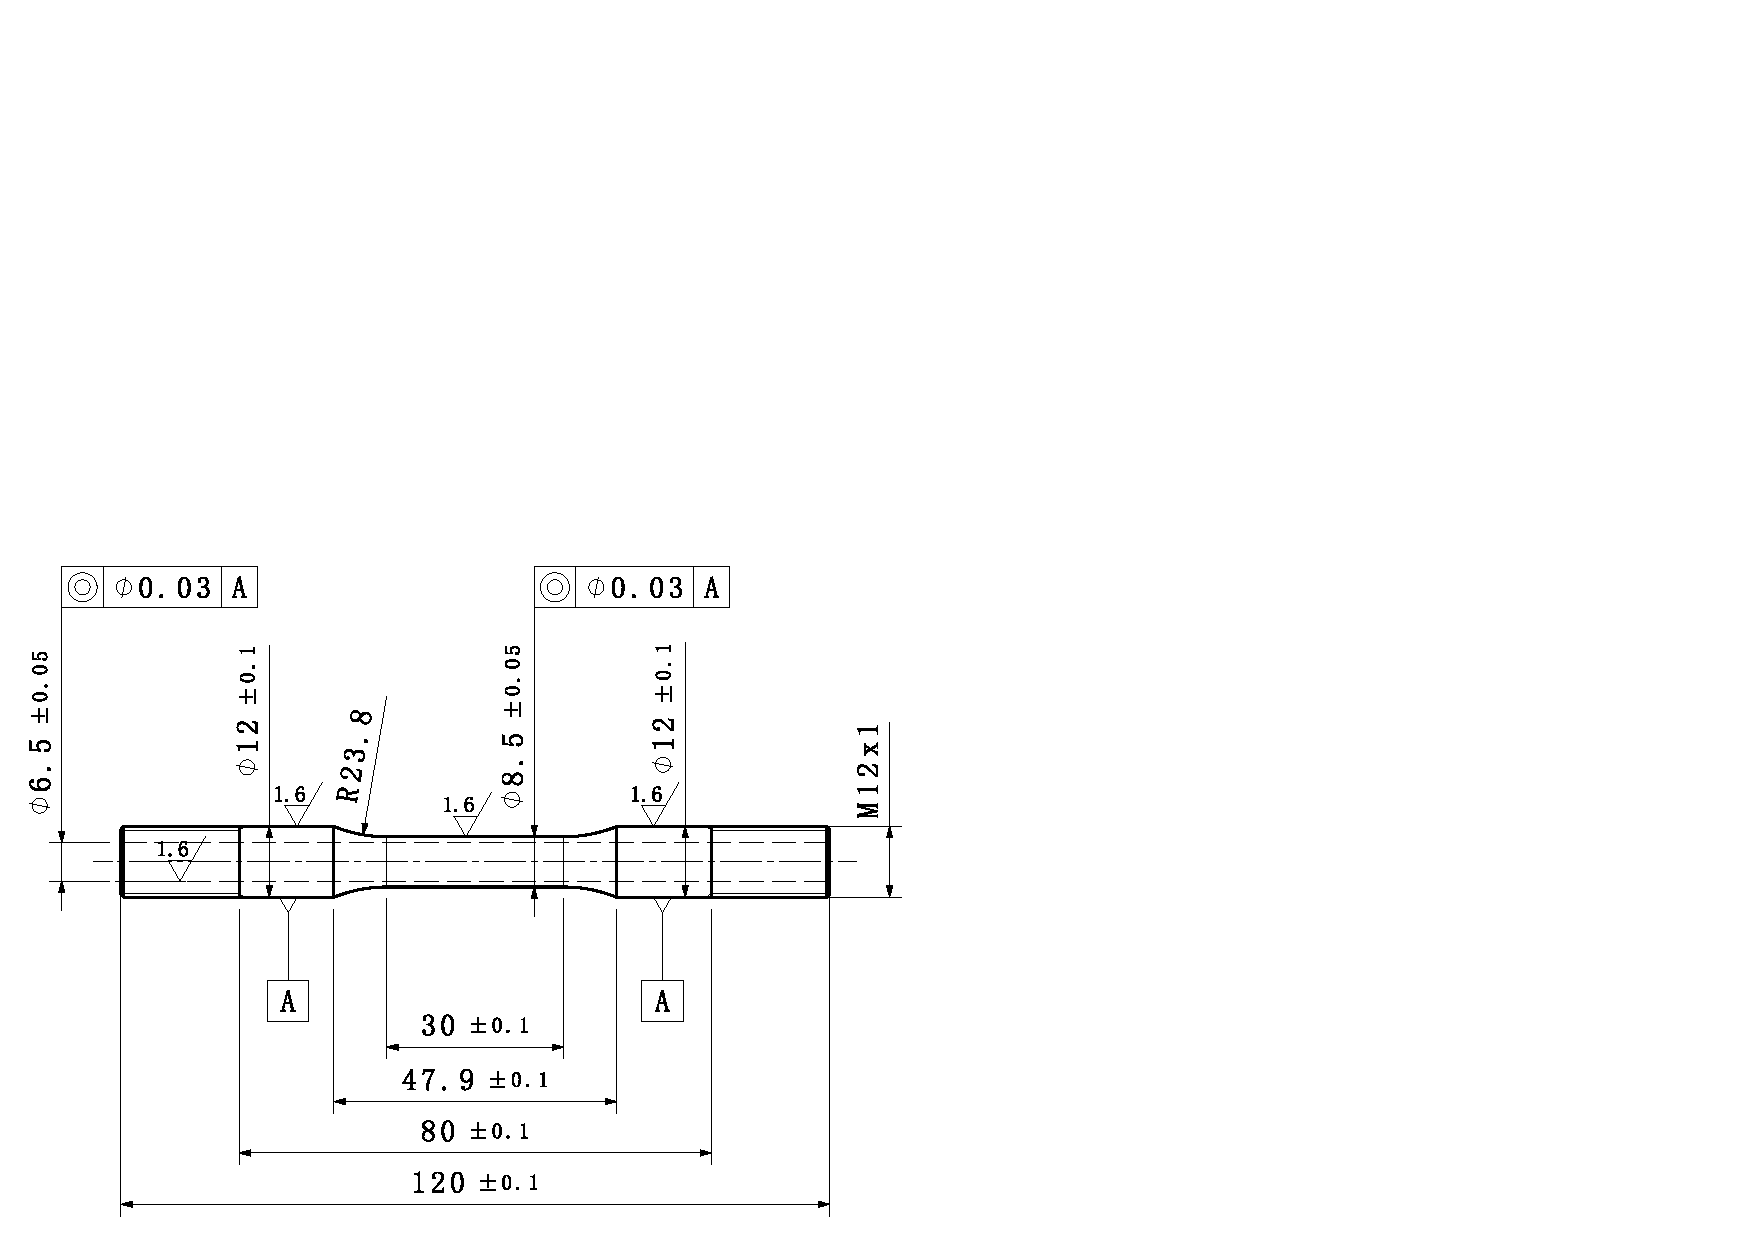
\includegraphics[width=10cm]{IN718_Axial_Specimen_TGMF.pdf}}
\caption{TGMF试样示意图.}
\label{Fig:Specimen}
\end{figure}

因此,参考德宇航的工作\cite{BAUFELD2008219},我们为热梯度机械疲劳(TGMF)测试设计开发了聚光辐射加热系统,如\ref{Fig:Radiation_Furnace2}所示。
该系统包括16根卤素灯管,灯丝的直径小于0.5mm,因此每根灯丝可以被抽象为一个线光源。
每根灯管对应一面反射镜,反射镜的几何形状为椭圆柱面,每根灯管位于其对应的椭圆柱面其中一个焦点,试件位于所有椭圆柱面的公共焦点,通过镜面反射将光线聚焦在试件表面进行加热。
通过聚光辐射的方法加热试件外表面,同时内表面通过压缩空气冷却来实现温度梯度。
该系统可以在空心试件表上实现受控的温度梯度循环,同时施加机械载荷,适用于金属和非金属材料。

在TMF和TGMF测试中,温度控制是实现每个测试的可重复加载条件的关键问题,两种试验采用相似的温度控制方法。
在测试过程中,使用接触式K型电偶测量试件外表面的温度,考虑到试验过程中温度变化速率很快,需要传感器对温度变化有迅速的响应,传感器体积越小,对温度的响应越迅速,因此我们选取测量点直径为0.25mm的热电偶,将试件中心点的温度作为控制量,以实现良好的温度控制,精度为±5°C。
对于试件内表面,考虑到气体流动,在TGMF期间,内部点焊热电偶是不可能的,因为它们的信号受到内部冷却的影响。
同时由于试件的尺寸很小,内孔直径只有6.5mm,也无法使用热像仪进行测量,因此在这里采用计算的方法来确定时间内表面的温度。
\begin{figure}[!htp]
\centering{\includegraphics[width=10cm]{Radiation_Furnace2.pdf}}
\caption{聚光辐射加热系统.}
\label{Fig:Radiation_Furnace2}
\end{figure}


\begin{table}[htbp]
  \centering
  \caption{650$^{\circ}$C恒温疲劳试验、TMF与TGMF试验结果.}
    \begin{tabular}{llllll}
    \toprule
    Test Type & $\pm \varepsilon _m$ & $\varepsilon _{eq}$ & $\dot \varepsilon _{eq}$ & $\theta_{T-\varepsilon}$ & $N_f$ \\
          & [\%]  & [\%]  & [s$^{-1}$] & [$^\circ$] &  \\
    \midrule
    IF & 1.00  & 1.00  & $1\times 10^{-3}$ & -     & 131 \\
          & 0.80  & 0.80  & $1\times 10^{-3}$ & -     & 326 \\
          & 0.70  & 0.70  & $1\times 10^{-3}$ & -     & 592 \\
          & 0.60  & 0.60  & $1\times 10^{-3}$ & -     & 1336 \\
          & 0.50  & 0.50  & $1\times 10^{-3}$ & -     & 8449 \\
          & 0.45  & 0.45  & $1\times 10^{-3}$ & -     & 15497 \\
          & 0.40  & 0.40  & $6.4\times 10^{-3}$ & -     & 130585 \\
    \midrule
    TMF-IP & 1.00  & 1.00  & $2.22\times 10^{-4}$ & 0     & 58 \\
          & 0.80  & 0.80  & $1.78\times 10^{-4}$ & 0     & 176 \\
          & 0.70  & 0.70  & $1.56\times 10^{-4}$ & 0     & 248 \\
          & 0.60  & 0.60  & $1.33\times 10^{-4}$ & 0     & 1297 \\
    \midrule
    TMF-OP & 1.00  & 1.00  & $2.22\times 10^{-4}$ & 180   & 209 \\
          & 0.80  & 0.80  & $1.78\times 10^{-4}$ & 180   & 303 \\
          & 0.70  & 0.70  & $1.56\times 10^{-4}$ & 180   & 429 \\
          & 0.65  & 0.65  & $1.44\times 10^{-4}$ & 180   & 633 \\
    \midrule
    TGMF-IP & 0.75  & 0.75  & $1.67\times 10^{-4}$ & 0     & 48 \\
          & 0.60  & 0.60  & $1.33\times 10^{-4}$ & 0     & 50 \\
          & 0.55  & 0.55  & $1.22\times 10^{-4}$ & 0     & 107 \\
          & 0.50  & 0.50  & $1.11\times 10^{-4}$ & 0     & 208 \\
          & 0.40  & 0.40  & $0.89\times 10^{-4}$ & 0     & 1066 \\
    \midrule
    TGMF-OP & 0.75  & 0.75  & $1.67\times 10^{-4}$ & 180   & 128 \\
          & 0.55  & 0.55  & $1.22\times 10^{-4}$ & 180   & 375 \\
          & 0.50  & 0.50  & $1.11\times 10^{-4}$ & 180   & 864 \\
          & 0.40  & 0.40  & $0.89\times 10^{-4}$ & 180   & 3387 \\
    \midrule
    TGMF-IP-TBC & 0.75  & 0.75  & $1.67\times 10^{-4}$ & 0     & 147 \\
          & 0.55  & 0.55  & $1.22\times 10^{-4}$ & 0     & 624 \\
    \bottomrule
    \end{tabular}%
  \label{tab:test_matrix}%
\end{table}%

\section{试验结果}

\begin{figure}
  \begin{minipage}[t]{0.5\linewidth} % 如果一行放2个图,用0.5,如果3个图,用0.33\
  \nonumber
    \centering
    \begin{overpic}[width=6.0cm]{plot_exp_half_life_cycle_TCIPTGMF.pdf}
      \put(0,65){\fcolorbox{white}{white}{(a)}}
    \end{overpic}
  \end{minipage}%
  \begin{minipage}[t]{0.5\linewidth}
    \centering
    \begin{overpic}[width=6.0cm]{plot_exp_half_life_cycle_TCOPTGMF.pdf}
      \put(0,65){\fcolorbox{white}{white}{(b)}}
    \end{overpic}
  \end{minipage}

  \caption{TGMF稳定滞后回线:(a)同相位,(b)反相位.}
  \label{Fig:plot_exp_half_life_cycle_TCTGMF}
\end{figure}

图\ref{Fig:plot_exp_half_life_cycle_TCTGMF}分别是同相位和反相位热梯度机械疲劳的稳定滞后回线。
由于热梯度机械疲劳的温度循环与载荷循环之间有相位差,导致其拉伸半周和压缩半周具有不同的循环软化行为。
对于同相位热梯度机械疲劳试验,合金在拉伸半周表现出较强的循环软化,而对于反相位热梯度机械疲劳试验则相反,合金在压缩半周表现出较强的循环软化。

\begin{figure}
  \begin{minipage}[t]{0.5\linewidth} % 如果一行放2个图,用0.5,如果3个图,用0.33\
  \nonumber
    \centering
    \begin{overpic}[width=6.0cm]{plot_exp_pv_TCIPTGMF.pdf}
      \put(0,65){\fcolorbox{white}{white}{(a)}}
    \end{overpic}
  \end{minipage}%
  \begin{minipage}[t]{0.5\linewidth}
    \centering
    \begin{overpic}[width=6.0cm]{plot_exp_pv_TCOPTGMF.pdf}
      \put(0,65){\fcolorbox{white}{white}{(b)}}
    \end{overpic}
  \end{minipage}

  \caption{TGMF应力均值与峰谷值:(a)同相位,(b)反相位.}
  \label{Fig:plot_exp_pv_TCTGMF}
\end{figure}

图\ref{Fig:plot_exp_pv_TCTGMF}分别是同相位和反相位热梯度机械疲劳的循环应力峰谷值和均值。
在所有的试验条件下,合金在最终断裂前循环应力峰谷值快速下降,这实际上是宏观裂纹的形成以及随后的失稳扩展至断裂的结果。
同相位和反相位热梯度机械疲劳试验均表现为循环软化,但温度循环与载荷循环之间的相位差,导致循环软化的程度不同,在300-650$^{\circ}$C范围内,温度越高,材料的循环软化越明显,因此对于同相位的情况,材料在拉伸半周的循环软化更强烈,反应在平均应力的演化上则表现为平均应力随着循环的增加,产生越来越大的平均压应力。

\begin{figure}
  \begin{minipage}[t]{0.5\linewidth} % 如果一行放2个图,用0.5,如果3个图,用0.33\
  \nonumber
    \centering
    \begin{overpic}[width=6.0cm]{plot_exp_mean_TCIPTGMF.pdf}
      \put(0,65){\fcolorbox{white}{white}{(a)}}
    \end{overpic}
  \end{minipage}%
  \begin{minipage}[t]{0.5\linewidth}
    \centering
    \begin{overpic}[width=6.0cm]{plot_exp_mean_TCOPTGMF.pdf}
      \put(0,65){\fcolorbox{white}{white}{(b)}}
    \end{overpic}
  \end{minipage}

  \caption{TGMF循环应力均值:(a)同相位,(b)反相位.}
  \label{Fig:plot_exp_mean_TCTGMF}
\end{figure}

平均应力是高温低周疲劳中不可忽视的因素,尤其对于强度较高而韧性较低的镍基高温合金而言,平均应力是影响疲劳寿命的重要因素,图\ref{Fig:plot_exp_mean_TCTGMF}所示为Inconel 718合金在同相位和反相位TGMF试验条件下的平均应力响应曲线。
可见,对于TGMF-IP,平均应力为压应力,机械应变幅的增加对平均应力的影响不大,对于不同的机械应变幅值,平均应力演化的速率相近,平均应力的数值随着循环数的增加而增大,
,当$\Delta_{\varepsilon}=0.4\%$时,半寿命时的压缩平均应力达65.9MPa(表3.1);对于oPTMF,平均应力为拉应力且随着机械应变幅的增加拉伸平均应力幅度变大,当v-耐/2=0.50\%时,半寿命时的拉伸平均应力约为102石MPa(3.2)"热机械疲劳中存在明显平均应力的原因是合金的强度随温度的不断变化"无论是同相位还是反相位热机械疲劳都经历低温到高温的温度循环,当试验温度较高时合金的强度较低,而当试验温度较低时合金的强度较高,因此造成了滞后回线的应力不对称性,平均应力总是偏向低温半周"而平均应力随机械应变幅增加而增大的原因是随着机械应变幅的增加,合金在高温半周产生的塑性变形增加,这加剧了拉压应力的不对称性"此外,可以观察到在两种TMF试验条件下平均应力幅值均随循环的进行而逐渐增大,这可认为是M963合金在高温半周持续循环软化以及低温半周持续循环硬化的综合作用结果"而对于900eIF试验,平均应力数值普遍较小,当v气-/2二0.50\%时,半寿命的平均应力仅约为一32.SMPa(表3.3),而对于更小的应变幅则平均应力接近为零,因此平均应力对900eIF试验的影响可以忽略"

\section{微观结构}



\section{Thermal gradient mechanical FE-analysis}

\subsection{冷却系统}


TGMF试验的试件内表面采用压缩空气进行冷却,冷却系统的结构如图\ref{Fig:inner_cooling}所示,包括空气压缩机、空气干燥器、流量计、压力表和流量控制器组成。
Because of the small inner diameter 6.5mm of the specimen, it is difficult to measure the temperature of the specimen inner surface during the tests.
A variety of measurement options were tried to measure the inner surface temperature.
It was found that the internal cooling air has a significant effect on the temperature measurement of the inner surface of the specimen.
%内部冷却空气对试件内壁的温度测量有很大的影响。
The measured temperature is not the temperature of the inner surface, but the average temperature of the wall and the cooling air flow.
%测量得到的温度不是壁面的温度,而是壁面和冷却气流的平均温度。
Therefore we tried to calculate the temperature distribution of the specimen inner surface using the FEM method.

%The internal diameter of the specimen is 6.5 mm, and .
%试件的内部直径为6.5mm,。
\begin{figure}[!htp]
\centering{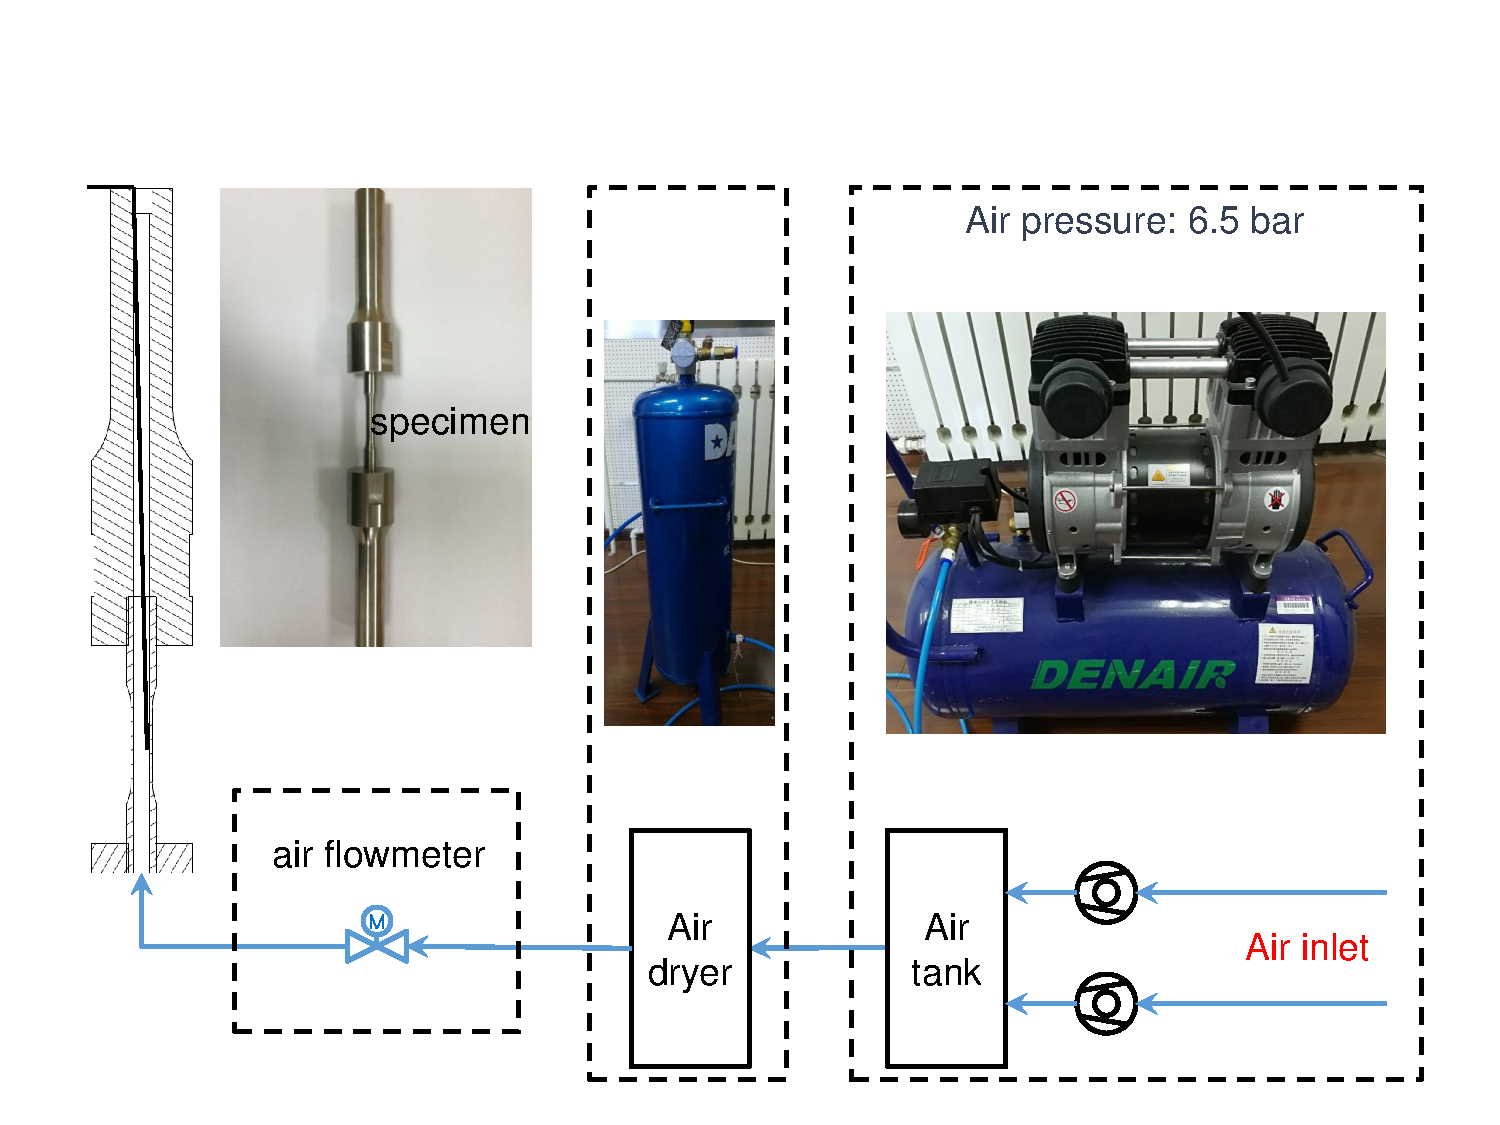
\includegraphics[width=12cm]{inner_cooling.pdf}}
\caption{Schematic of inner cooling air system.}
\label{Fig:inner_cooling}
\end{figure}

\subsection{Model description}
TGMF试件的几何形状如图\ref{Fig:Specimen}所示,由于几何形状和外部环境的对称性,我们取出试样的标距段部分,建立轴对称有限元模型,如图\ref{Fig:FEM}所示,标距段长度为12mm,取试件的中心界面作为轴对称面。
用以下物理边界条件进行辐射加热的TGMF试样几何形状的有限元分析:
试件外表面为温度边界,随时间变化的温度分布可由试验测得,试件内表面为对流边界条件,对流换热系数由圆管强制对流换热公式计算,需要试验测量冷却空气的密度、温度和体积流量。由于试件的对称性,中心对称界面可假设为绝热边界。
试件的上边界认为是热传导边界,热传导系数。
试件表面的发射率$\varepsilon=0.75$

\begin{figure}[!htp]
\centering{\includegraphics[width=12cm]{FEM.pdf}}
\caption{Simulated temperature distribution and resulting axial stress component during heating of an inductively heated TMF specimen.}
\label{Fig:FEM}
\end{figure}

\begin{figure}[!htp]
\centering{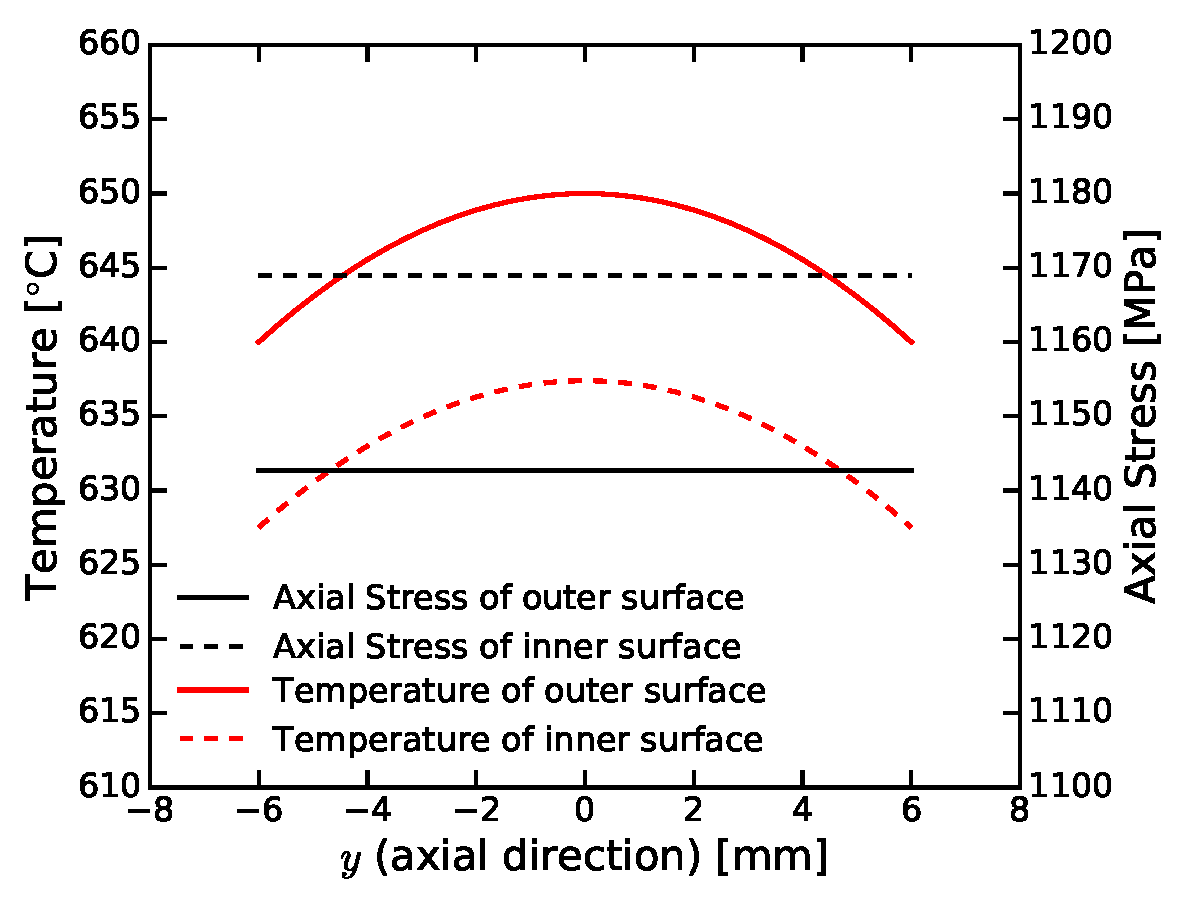
\includegraphics[width=12cm]{plot_temperature_along_gauge_length.pdf}}
\caption{Diagram of simulated axial temperature gradients and the resulting, thermally induced axial stress components at maximum temprature (650$^{\circ}$C) during TGMF tests.}
\label{Fig:plot_temperature_along_gauge_length}
\end{figure}

\begin{figure}[!htp]
\centering{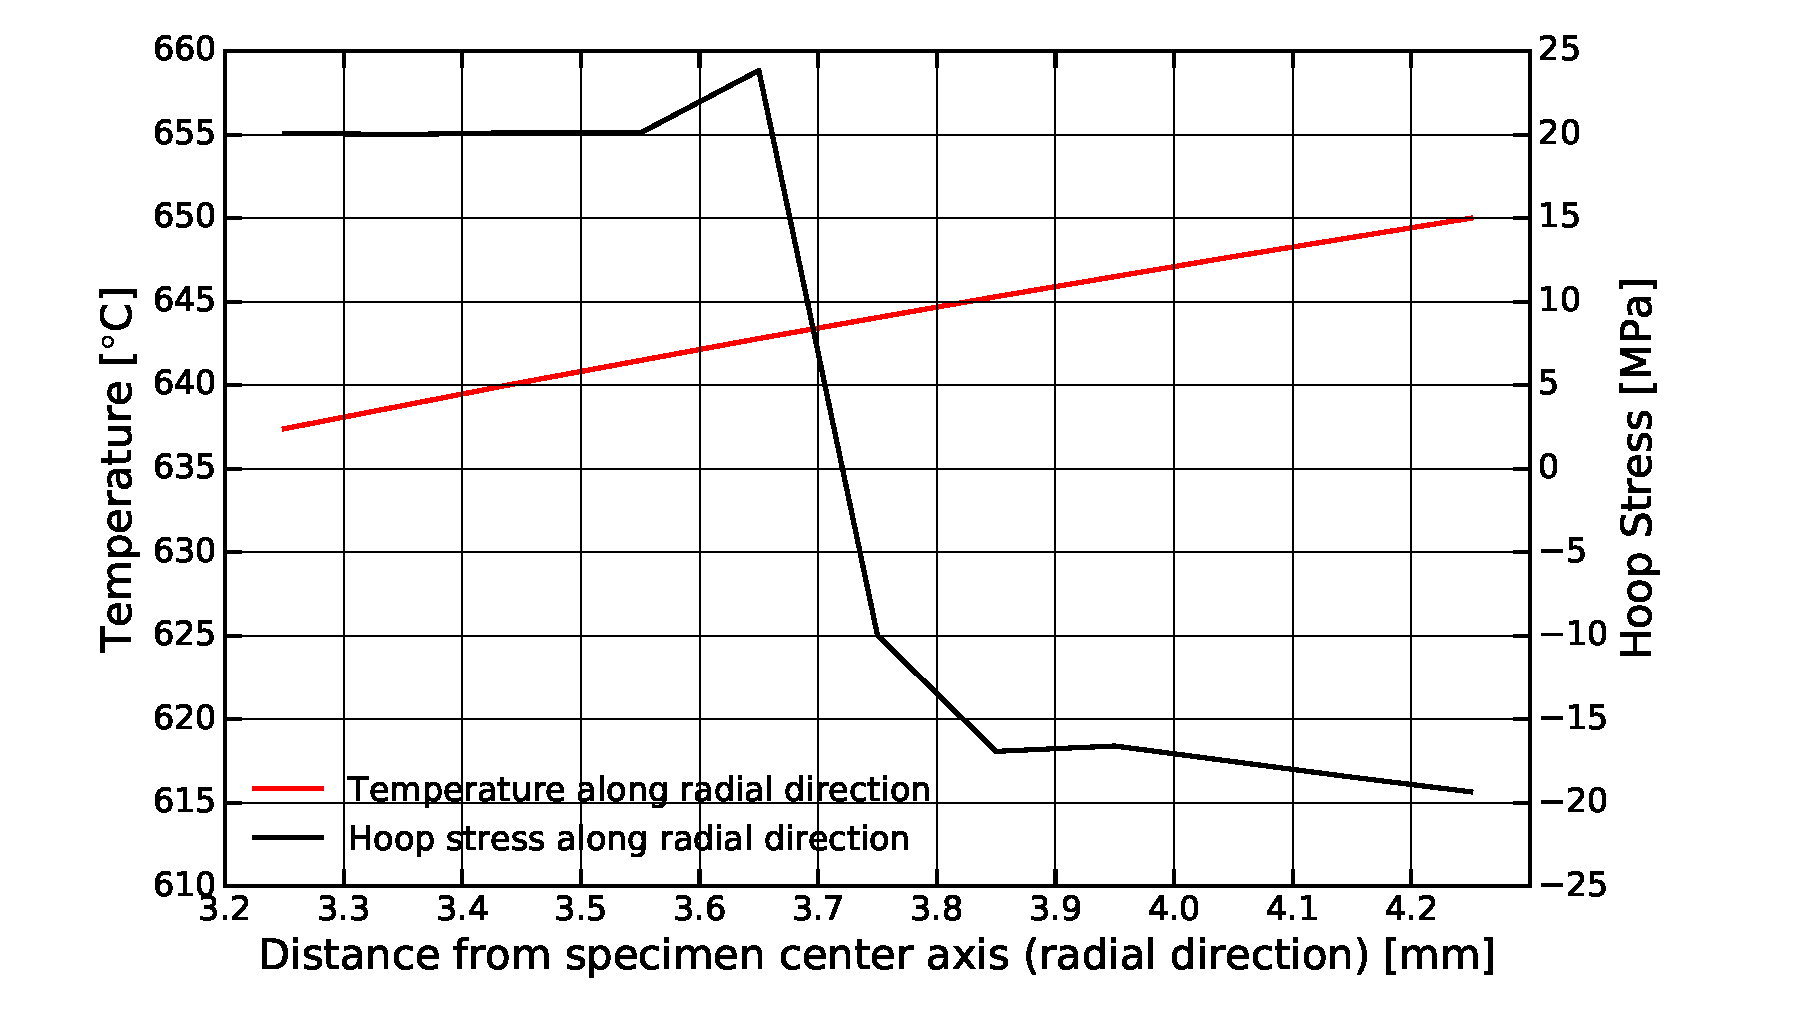
\includegraphics[width=12cm]{plot_temperature_along_radial_direction.pdf}}
\caption{Diagram of simulated radial temperature gradients and the resulting, thermally induced hoop stress components at maximum temprature (650$^{\circ}$C) during TGMF tests.}
\label{Fig:plot_temperature_along_radial_direction}
\end{figure}




The inner surface of the hollow specimen can be considers as a pipe.
%空心试件可以简化为圆管.
According to the formula of convection in turbulent pipe flow, the convective heat transfer coefficient of the inner surface of the specimen can be calculated.
%根据圆管内部的强制对流换热公式,我们计算试件内表面的对流换热系数。

Nusselt number (Nu) is a dimensionless number, defined as the ratio of convective to conductive heat transfer across (normal to) the boundary.
The Nusselt number is given as:
\[{\rm{N}}{{\rm{u}}_L} = \frac{{hL}}{k},\]
where $h$ is the convective heat transfer coefficient of the fluid, $L$ is the characteristic length, $k$ is the thermal conductivity of the fluid.

Gnielinski's correlation for turbulent flow in tubes is given as:
\[{\rm{N}}{{\rm{u}}_D} = \frac{{\left( {f/8} \right)\left( {{\rm{R}}{{\rm{e}}_D} - 1000} \right){\rm{Pr}}}}{{1 + 12.7{{(f/8)}^{1/2}}\left( {{\rm{P}}{{\rm{r}}^{2/3}} - 1} \right)}},\]
where $f$ is the Darcy friction factor that can either be obtained from the Moody chart or for smooth tubes from correlation developed by Petukhov:
\[f = {\left( {0.79\ln \left( {{\rm{R}}{{\rm{e}}_D}} \right) - 1.64} \right)^{ - 2}},\]
with
\[0.5 \le {\rm{Pr}} \le 2000,\]
\[3000 \le {\rm{R}}{{\rm{e}}_D} \le 5 \times {10^6},\]

The Prandtl number (Pr) is a dimensionless number, defined as the ratio of momentum diffusivity to thermal diffusivity.
The Prandtl number is given as:
\[{\rm{Pr}} = \frac{{{c_p}\mu }}{k},\]
where
$c_{p}$ is specific heat, $\mu$ is dynamic viscosity and $k$ is thermal conductivity.

The Reynolds number (Re) is a dimensionless number, defined as the ratio of inertial forces to viscous forces within a fluid.
The Reynolds number is given as:
\[{\rm{Re}} = \frac{{\rho uL}}{\mu },\]
where
$\rho$ is density of the fluid, $u$ is the velocity of the fluid with respect to the object, $\mu$ is the dynamic viscosity of the fluid and $L$ is a characteristic dimension.

It is noted that the dynamic viscosity $\mu$ of an ideal gas is a function of the temperature. It can be derived as Sutherland's formula:
\[\mu  = {\mu _0}\frac{{{T_0} + C}}{{T + C}}{\left( {\frac{T}{{{T_0}}}} \right)^{\frac{3}{2}}},\]
where $\mu$ is dynamic viscosity at input temperature $T$,
$\mu_0$ is reference viscosity at reference temperature $T_0$,
$C$ is Sutherland's constant dependent on the gaseous material.
Table \ref{tab:SutherlandConstant} shows the Sutherland's constant and reference values of the air.
\begin{table}[htbp]
  \centering
  \caption{Sutherland's constant and reference values of the air.}
    \begin{tabular}{p{2cm}p{2cm}p{2cm}p{3cm}}
    \toprule
    Gas   & $C$(K) & $T_0$(K) & $\mu_0$($\rm{Pa\cdot s}$) \\
    \midrule
    air   & 120   & 291.15 & $1.827\times 10^{-5}$ \\
    \bottomrule
    \end{tabular}%
  \label{tab:SutherlandConstant}%
\end{table}%

The density of dry air $\rho$ can be calculated using the ideal gas law, expressed as a function of temperature and pressure:
\begin{equation}
\rho  = \frac{p}{{RT}},
\label{Equ:AirDensity}
\end{equation}
where
$p$ is absolute pressure,
$T$ is absolute temperature,
$R$ is specific gas constant.

According to the measurement results of the sensors, the average pressure and temperature of the cooling air are 6.5 bar and 288.15K, respectively.

\begin{table}[htbp]
  \begin{threeparttable}
  \centering
  \caption{Heat convection coefficients of the inner surface of the specimen.}
    \begin{tabular}{llrrrr}
    \toprule
    $T$   & ${\rm{K}}$ & 288.15  & 288.15  & 288.15  & 288.15  \\
    $p$   & ${\rm{bar}}$ & 6.5   & 6.5   & 6.5   & 6.5  \\
    $\rho  = \frac{p}{{RT}}$ \tnote{*1} & ${\rm{kg/}}{{\rm{m}}^{\rm{3}}}$ & 7.724 & 7.724 & 7.724 & 7.724 \\
    $\mu  = {\mu _0}\frac{{{T_0} + C}}{{T + C}}{\left( {\frac{T}{{{T_0}}}} \right)^{\frac{3}{2}}}$ \tnote{*2} & -     & 1.81E-05 & 1.81E-05 & 1.81E-05 & 1.81E-05 \\
    ${\dot V}$ & ${\rm{l/min}}$ & 10    & 20    & 30    & 40  \\
    $u = \frac{{4\dot V}}{{\pi {D^2}}}$ \tnote{*3} & ${\rm{m/}}{{\rm{s}}^2}$ & 5.02  & 10.05  & 15.07  & 20.09  \\
    ${\rm{Re}} = \frac{{\rho uL}}{\mu }$ \tnote{*4} & -     & 13906  & 27812  & 41718  & 55624  \\
    ${\rm{Pr}} = \frac{{{c_p}\mu }}{k}$ \tnote{*5} & -     & 0.63  & 0.63  & 0.63  & 0.63  \\
    $f = {\left( {0.79\ln \left( {{\rm{R}}{{\rm{e}}_D}} \right) - 1.64} \right)^{ - 2}}$ & -     & 0.0288  & 0.0241  & 0.0219  & 0.0205  \\
    ${\rm{N}}{{\rm{u}}_D} = \frac{{\left( {f/8} \right)\left( {{\rm{R}}{{\rm{e}}_D} - 1000} \right){\rm{Pr}}}}{{1 + 12.7{{(f/8)}^{1/2}}\left( {{\rm{P}}{{\rm{r}}^{2/3}} - 1} \right)}}$ & -     & 36.76  & 62.61  & 85.39  & 106.50  \\
    $h = \frac{k}{{D{\rm{N}}{{\rm{u}}_D}}}$ & ${\rm{W/(}}{{\rm{m}}^{\rm{2}}} \cdot {\rm{K)}}$ & 146.03  & 248.74  & 339.24  & 423.10  \\
    \bottomrule
    \end{tabular}%
    \begin{tablenotes}
    \item[*1] $R = 287.058 {\rm{J/(kg}} \cdot {\rm{K}})$ for dry air.
    \item[*2] Sutherland's constant and reference values of the air (see Table \ref{tab:SutherlandConstant}).
    \item[*3] $D=0.65$mm.
    \item[*4] $L=D$.
    \item[*5] $c_{p}=903.3 {\rm{J/(kg}} \cdot {\rm{K}})$ and $k=0.0258 {\rm{W/(m}} \cdot {\rm{K}})$ at $288.15{\rm{K}}$.
    \end{tablenotes}
    \end{threeparttable}
  \label{tab:addlabel}%
\end{table}%

\section{寿命预测}
\subsection{试验结果}
TGMF是一个复杂的试验状态,对于圆管试件,温度梯度导致试件径向与轴向产生额外应力,试件内表面的温度低,表现为多轴拉伸载荷,与之相反,试件外表面的温度高,表现为多轴压缩载荷。
同时由于温度梯度的存在,导致材料的力学性能在径向方向有所区别,这会导致材料在试验过程中的塑性应变累积有所不同,我们无法通过试验观测,只能通过合适的本构模型进行计算。
通过对疲劳端口的观察,我们发现裂纹的萌生都是由外表面开始的,
如图\ref{Fig:plot_exp_fatigue_life}所示,我们发现对于无涂层的试件,TGMF的寿命要明显低于TMF的寿命,更大大低于恒温疲劳的寿命。

在机械应变控制条件下,一般可以通过机械应变幅与疲劳寿命之间的关系来考查材料的热机械疲劳寿命行为。图\ref{Fig:plot_exp_fatigue_life}所示为同相位、反相位热机械疲劳和650$^{\circ}$C等温疲劳试验条件下机械应变与疲劳寿命之间的关系。可见300-650$^{\circ}$C的热机械疲劳比℃的等温疲劳具有更大的损伤。在同等机械应变幅下℃等温低周疲劳具有较高的疲劳寿命,而和则寿命较低,且、机械应变幅一寿命关系曲线存在相互交叉,交叉点的位置大概在机械应变幅为左右。当机械应变幅较高时,同相位热机械疲劳倾向于具有较低的疲劳寿命而当机械应变幅较低时,反相位热机械疲劳倾向于具有较低的疲劳寿命
\begin{figure}[!htp]
\centering{\includegraphics[width=10cm]{plot_exp_fatigue_life.pdf}}
\caption{恒温试验(IF)、热机械疲劳试验(TMF)和热梯度机械疲劳试验(TGMF)寿命比较.}
\label{Fig:plot_exp_fatigue_life}
\end{figure}

\subsection{微观结构}

\subsection{疲劳模型}
(1)W-B模型


(2)F-S模型
The following models have been selected to the analysis:
 non-energetic stress-strain Fatemi-Socie model, based on the critical plane approach [22,23]

与应力准则相对应,早期的研究者Yokobori等将静强度理论应用到多轴应变准则中来。
采用最大法向应变、最大剪应变、Von Mises等效应变等代替Manson-Coffin公式的应变,与单轴低周疲劳估算相似,进行多轴疲劳寿命预算。
由于该方法没有考虑不同应力路径对材料响应和疲劳寿命的影响,因而不能用于预测多轴非比例加载下的疲劳寿命。

Brown和Miller[31]根据疲劳裂纹萌生和扩展的物理解释提出了一种多轴疲劳理论,与Findley[17-20]提出的应力准则相类似,Brown和Miller认为最大剪平面上的剪应变和法向应变这两个参数都应该考虑。他们提出裂纹第一阶段沿最大剪切面生成,第二阶段沿垂直于最大拉应变方向扩展。
Brown和Miller准则由一系列由最大剪应变${\gamma _{\max }}$和最大剪应变平面上的法向应变${\varepsilon _n}$为坐标所组成的$\Gamma$平面上的等寿命曲线组成,对于给定寿命有
\[{\gamma _{\max }} = f\left( {{\varepsilon _n}} \right)\]

上式对于A、B两类裂纹有着不同的表达式。Brown和Miller将裂纹分为两种情况。在复合拉伸和扭转中,主应变${\varepsilon _1}$和${\varepsilon _3}$平行于表面,裂纹沿着表面扩展称为A类裂纹;对于正的双向拉伸,应变${\varepsilon _3}$垂直于自由表面,裂纹在自由表面上萌生进而沿纵深方向扩展称为B类裂纹。
Kandil,Brown和Miller[32]给出A类裂纹表达式的简化形式:
\[\frac{{\Delta {\gamma _{\max }}}}{2} + k\Delta {\varepsilon _n} = C\]
其中,$\Delta {\varepsilon _n}$是临界面上的法向应变变幅,$k$和$C$是材料常数。这一准则被广泛讨论及应用[33-36]。

Wang和Brown[37]用相邻两个最大剪应变折返点之间的法向应变变程${\varepsilon _n^*}$来代替法向应变变程$\Delta {\varepsilon _n}$,给出疲劳破坏模型
\[\frac{{\Delta {\gamma _{\max }}}}{2} + k\varepsilon _n^* = C\]
其中$k$和$C$是材料常数。

Fatemi和Socie[38]研究后发现,由于Kandil、Brown和Miller破坏模型的参数都是应变,没有考虑非比例加载下由于主轴旋转所产生的附加强化效
应,所以预测的多轴非比例加载下的疲劳寿命偏于危险,建议以最大剪应变平面上的最大法向应力${\sigma _{n,\max }}$
代替法向应变变程$\Delta {\varepsilon _n}$作为参数,提出准则如下:
\[\frac{{\Delta {\gamma _{\max }}}}{2}\left( {1 + k\frac{{{\sigma _{n,\max }}}}{{{\sigma _y}}}} \right) = C\]

\subsection{Brown-Miller Model}

1973年Brown和Miller\cite{Brown1973}根据疲劳裂纹扩展的物理解释提出了一种多轴疲劳模型,以最大剪切应变$\Delta\gamma_{max}$和最大剪切应变平面上的法向应变$\varepsilon_{n,max}$作为疲劳损伤参量。
1977年Kanazawa等\cite{KANAZAWA1979}对一批不锈钢进行了不同幅值比值和相位角的双轴拉扭试验,对最大剪应变平面上的正应变幅进行了观察,认为其面上正应变和剪应变之间的相位差对疲劳寿命没影响,故采用正应变幅和剪应变幅作为寿命拟合参数。
1993年Wang C. H.、Brown M. W.提出了一种考虑最大剪应变幅和最大剪应变幅平面上正应变程的多轴疲劳寿命模型,仅一个试验参数,可由单轴拉伸试验和扭转试验来确定[155]。
其考虑正应变变程的寿命计算公式(简称WB模型)为:
\[\frac{{\Delta {\gamma _{{\rm{max}}}}}}{2} + S{\varepsilon _{{\rm{n,max}}}} = \left[ {1 + {\nu _{\rm{e}}} + \left( {1 + {\nu _{\rm{e}}}} \right)S} \right]\frac{{{{\sigma '}_f}}}{E}{\left( {2{N_f}} \right)^b} + \left[ {1 + {\nu _{\rm{p}}} + \left( {1 + {\nu _{\rm{p}}}} \right)S} \right]{\varepsilon '_f}{\left( {2{N_f}} \right)^c}\]
其中,$\Delta\gamma_{max}$为最大剪应变平面上的剪应变幅,$\epsilon_{n,max}$为垂直最大剪应变平面上的最大正应变程,$S$为材料常数,$\nu_e$为弹性泊松比,$\nu_p$为塑性泊松比。
一般地,参数$S$不是常数,它会随疲劳寿命不同而改变。

\begin{figure}[!htp]
\centering{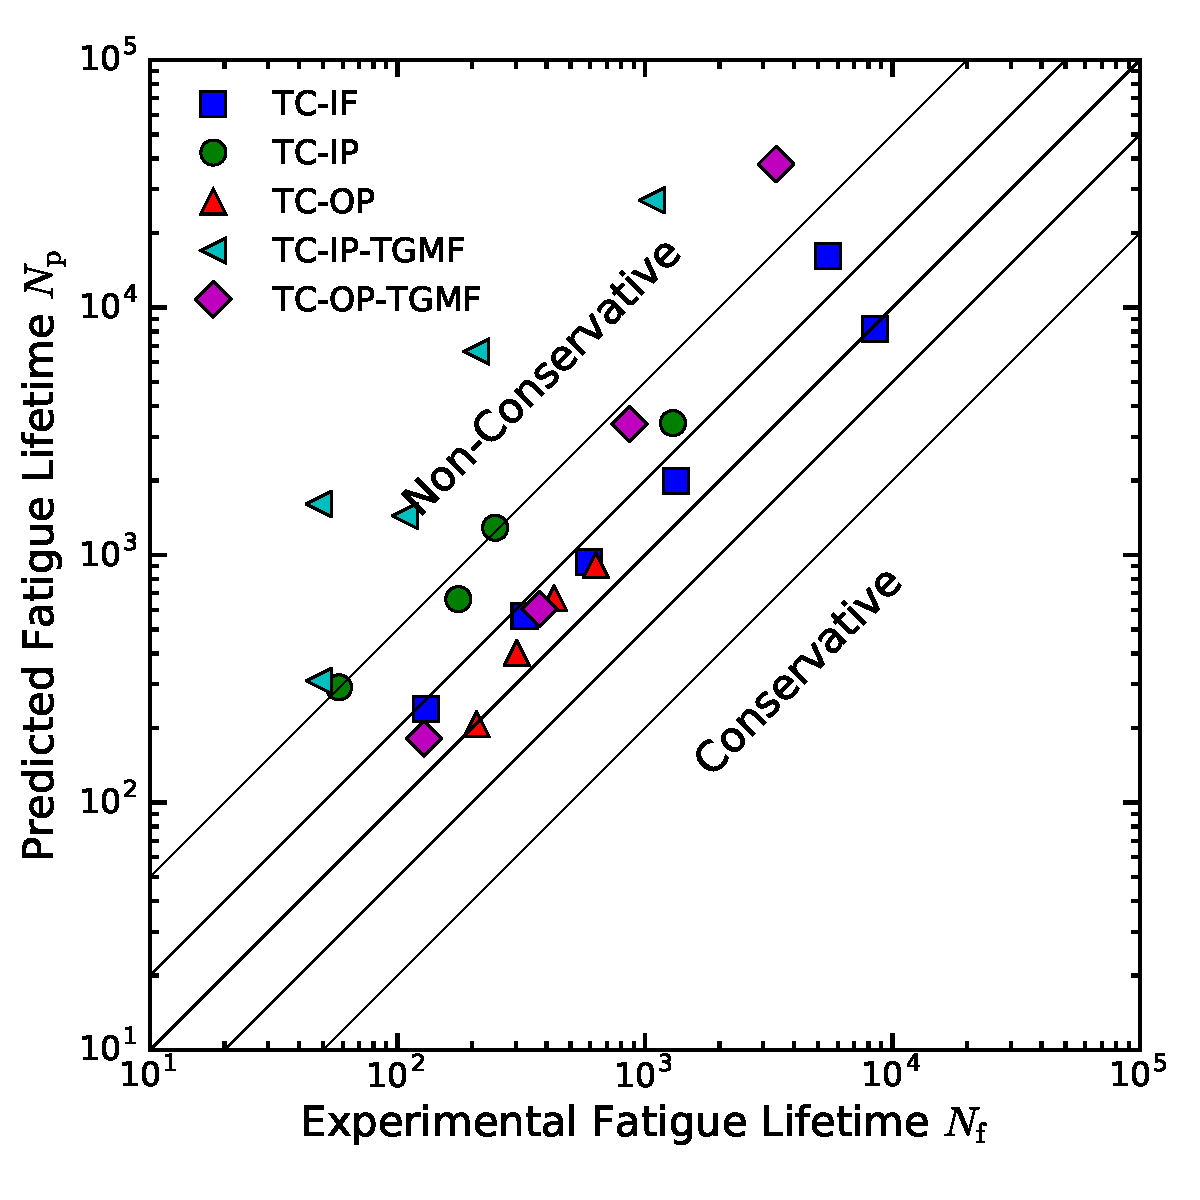
\includegraphics[width=8.5cm]{NF-NP-TGMF-BM.pdf}}
\caption{Fatemi-Socie Model.}
\label{Fig:NF-NP-TGMF-BM}
\end{figure}

\subsection{Fatemi-Socie Model}

\begin{figure}[!htp]
\centering{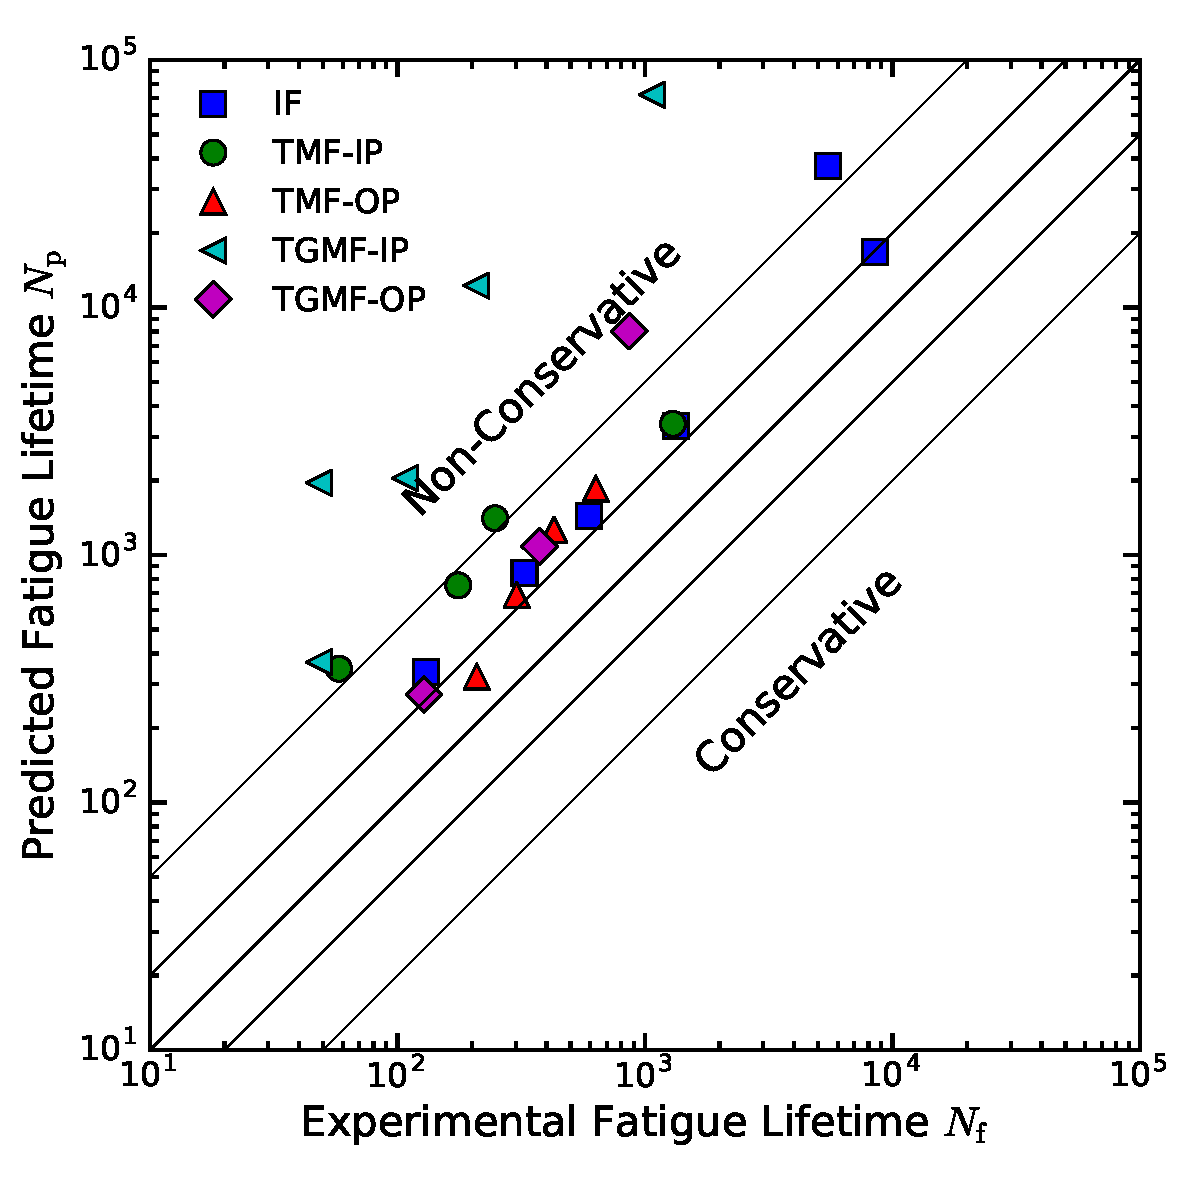
\includegraphics[width=8.5cm]{NF-NP-TGMF-FS.pdf}}
\caption{Fatemi-Socie Model.}
\label{Fig:NF-NP-TGMF-FS}
\end{figure}

\subsection{Smith-Watson-Topper Model}

\begin{figure}[!htp]
\centering{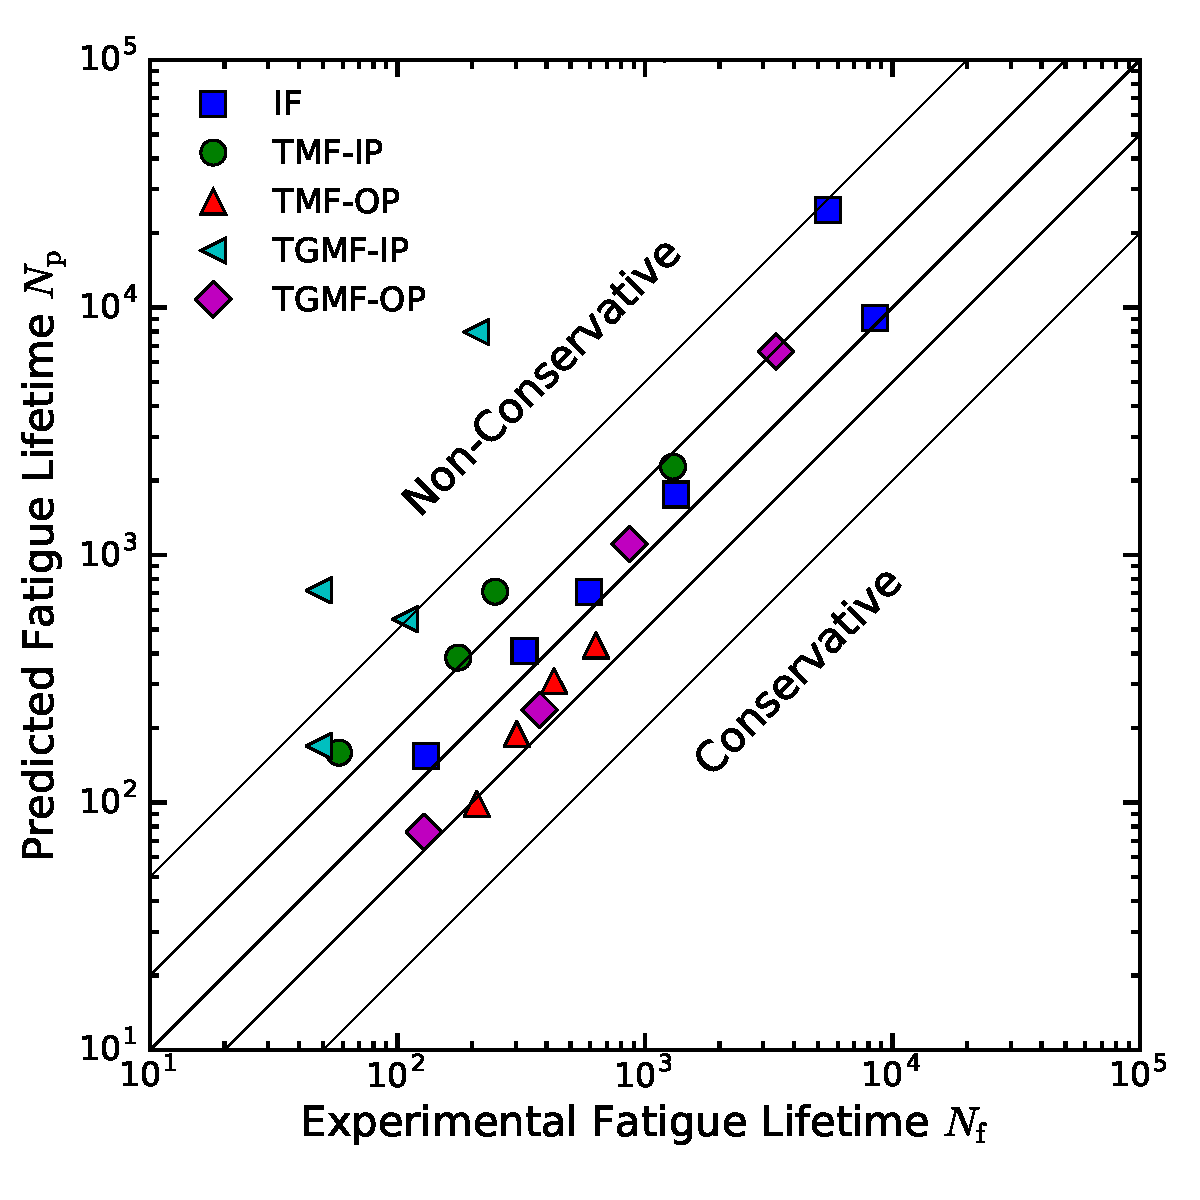
\includegraphics[width=8.5cm]{NF-NP-TGMF-SWT.pdf}}
\caption{Smith-Watson-Topper Model.}
\label{Fig:NF-NP-TGMF-SWT}
\end{figure}

\subsection{Liu’s Strain Energy Models}

\begin{figure}[!htp]
\centering{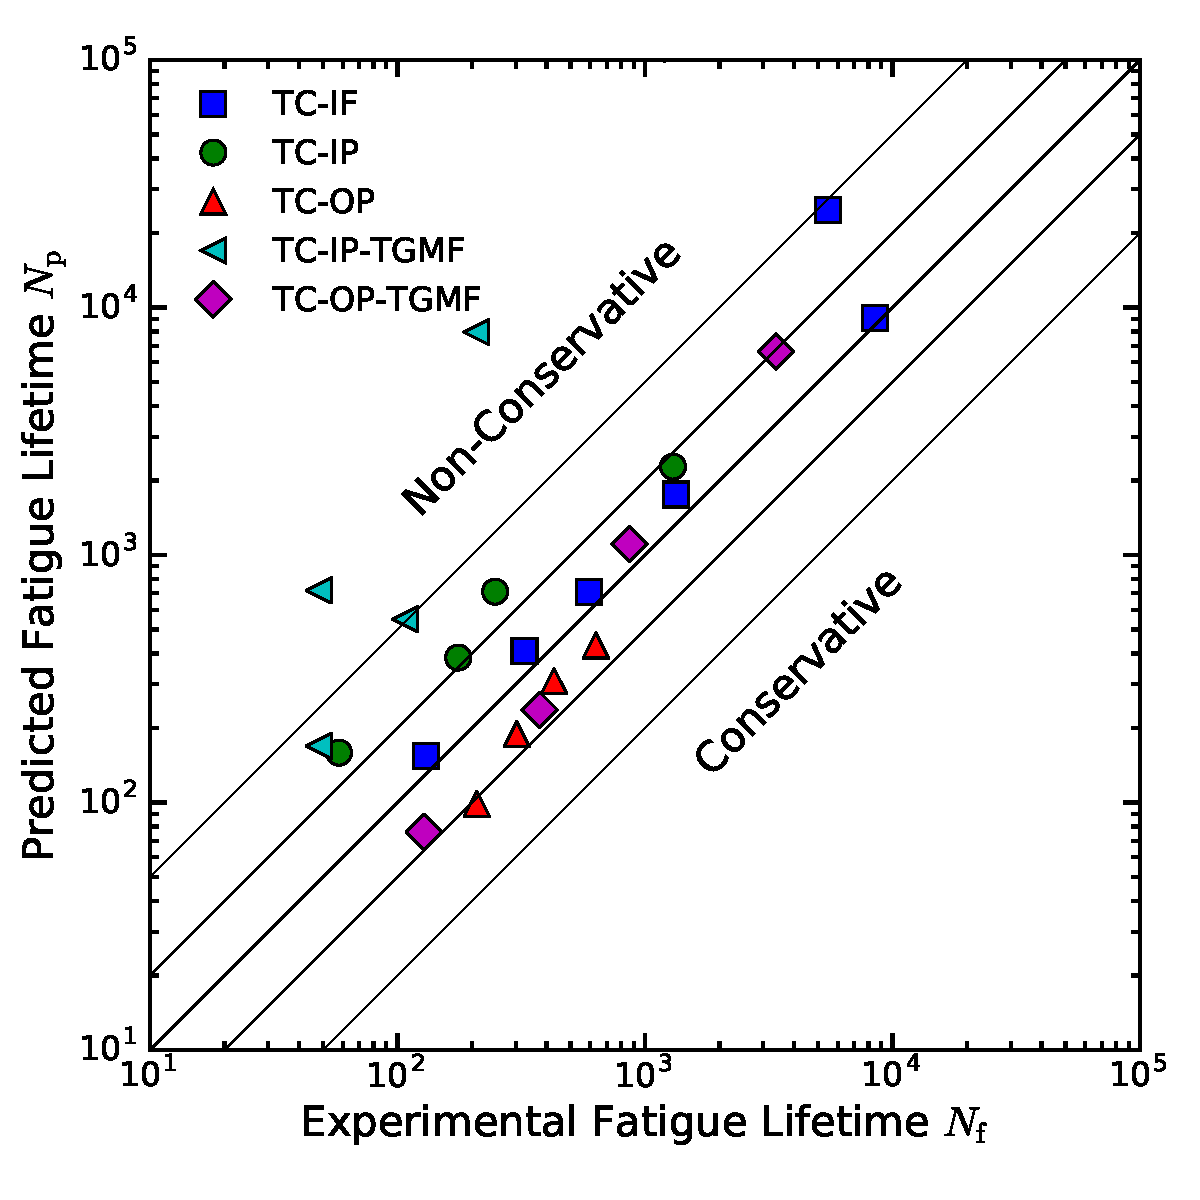
\includegraphics[width=8.5cm]{NF-NP-TGMF-Liu1.pdf}}
\caption{Liu Tension Strain Energy Model.}
\label{Fig:NF-NP-TGMF-Liu1}
\end{figure}

\begin{figure}[!htp]
\centering{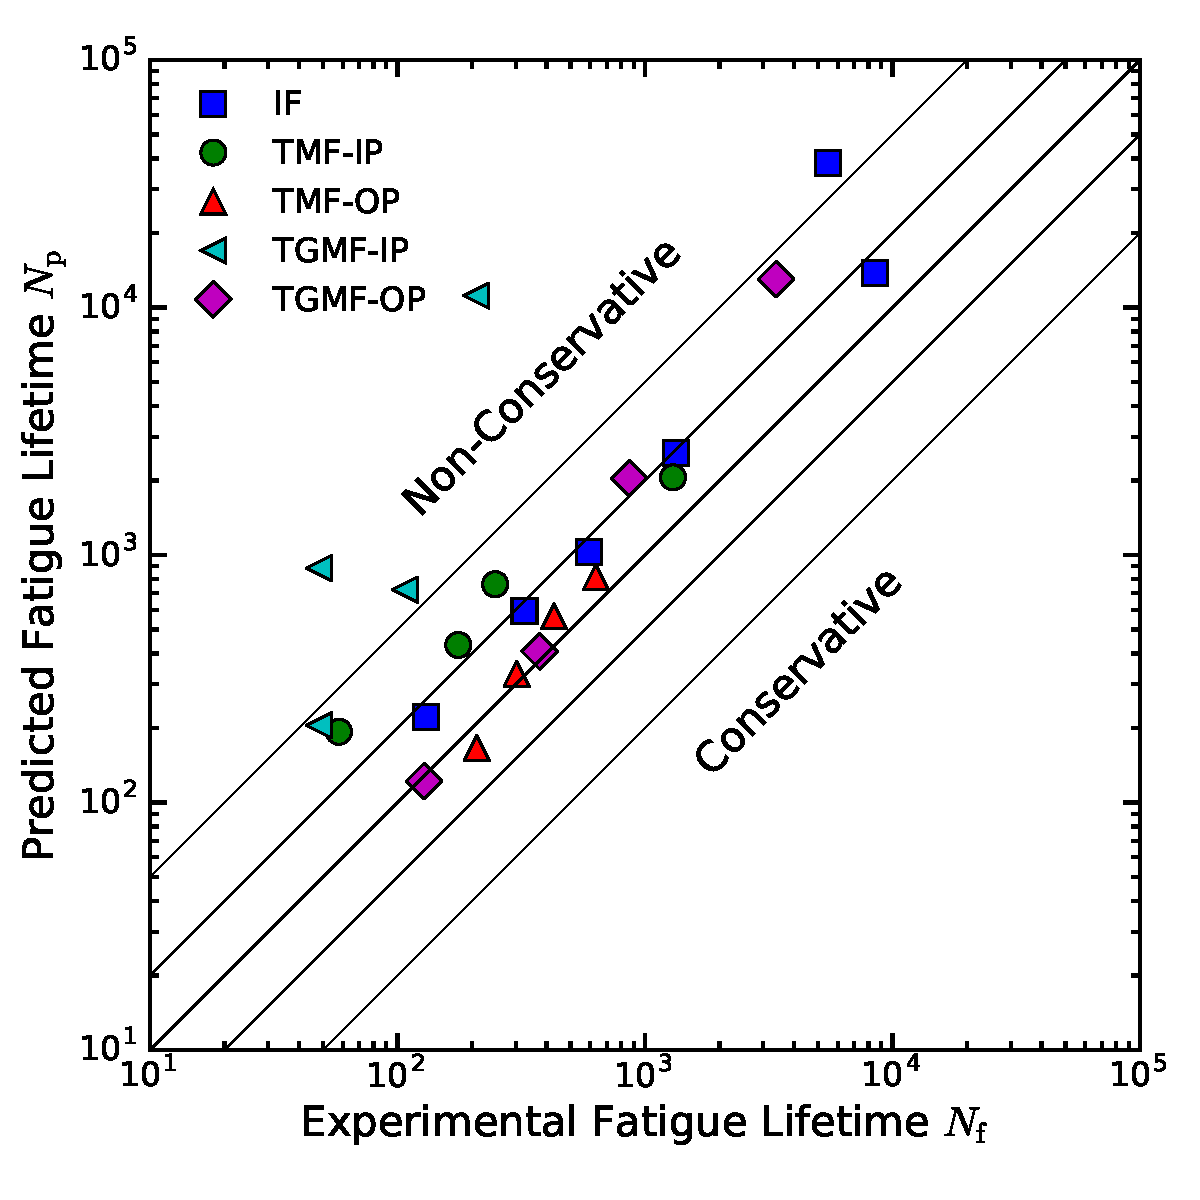
\includegraphics[width=8.5cm]{NF-NP-TGMF-Liu2.pdf}}
\caption{Liu Shear Strain Energy Model.}
\label{Fig:NF-NP-TGMF-Liu2}
\end{figure}

\subsection{Chu Strain Energy Model}
\begin{figure}[!htp]
\centering{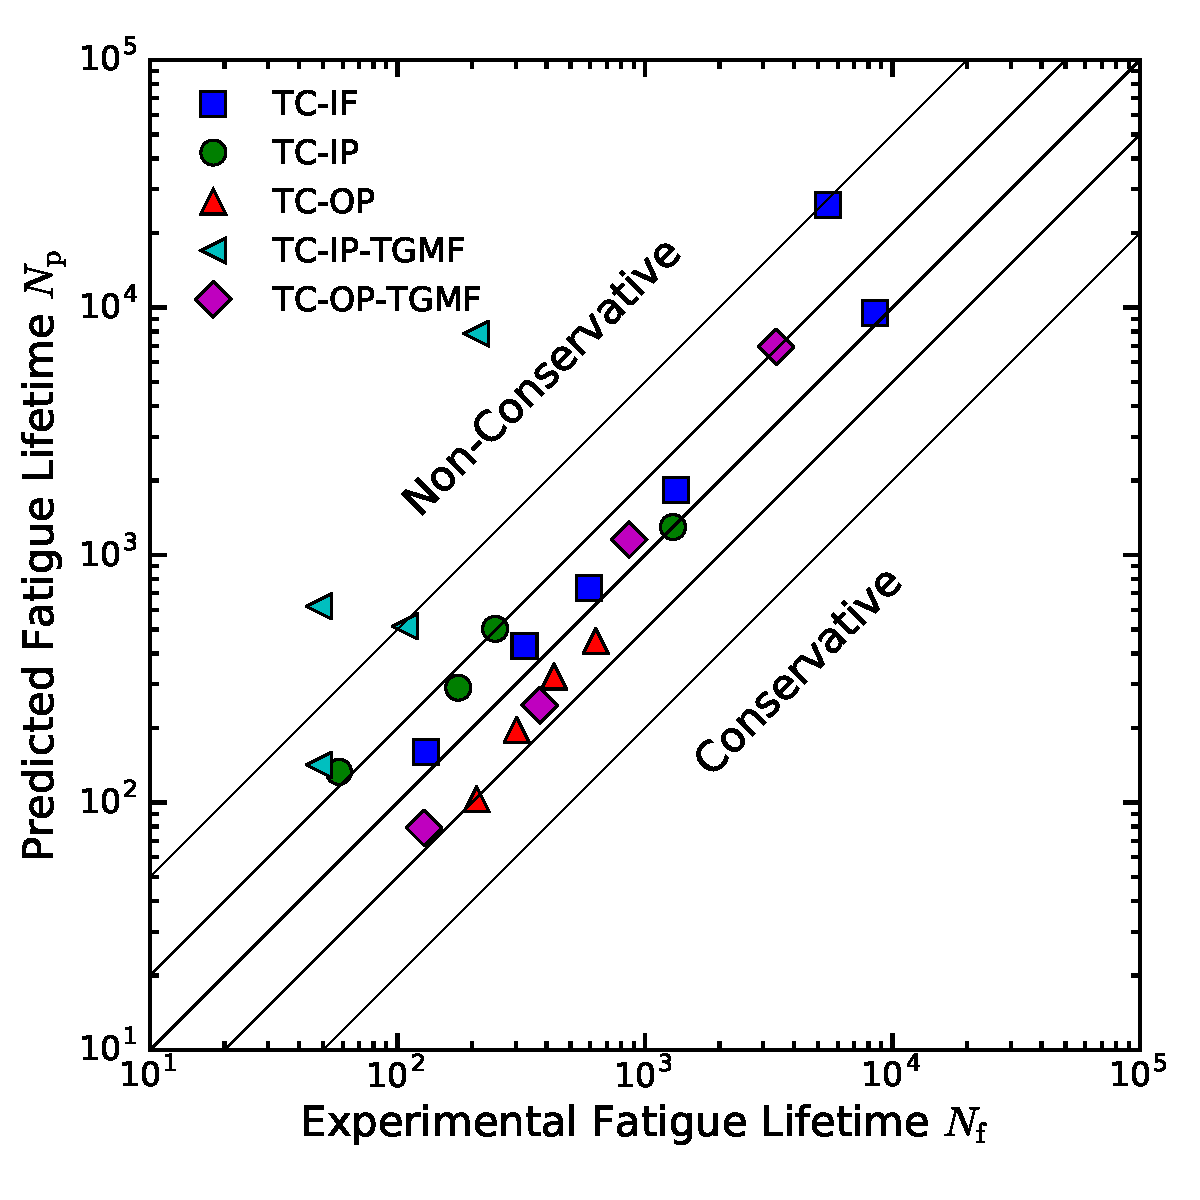
\includegraphics[width=8.5cm]{NF-NP-TGMF-Chu.pdf}}
\caption{Chu Strain Energy Model.}
\label{Fig:NF-NP-TGMF-Chu}
\end{figure}

% \begin{figure}
%   \begin{minipage}[t]{0.5\linewidth}
%   \nonumber
%     \centering
%     \includegraphics[width=6cm]{7033-1.jpg}
%     \centerline{(a)500X.}
%   \end{minipage}%
%   \begin{minipage}[t]{0.5\linewidth}
%     \centering
%     \includegraphics[width=6cm]{7033-12.jpg}
%     \centerline{(b)850.}
%   \end{minipage}
%   \caption{TC-OP.}
%   \label{Fig:MicrostructureofInconel718}
% \end{figure}

% \begin{figure}
%   \begin{minipage}[t]{0.5\linewidth}
%   \nonumber
%     \centering
%     \includegraphics[width=6cm]{7036-1.jpg}
%     \centerline{(a)$\Delta \varepsilon_{m}/2=0.5\%$.}
%   \end{minipage}%
%   \begin{minipage}[t]{0.5\linewidth}
%     \centering
%     \includegraphics[width=6cm]{7036-7.jpg}
%     \centerline{(b)$\Delta \varepsilon_{m}/2=0.5\%$.}
%   \end{minipage}

%   \begin{minipage}[t]{0.5\linewidth}
%   \nonumber
%     \centering
%     \includegraphics[width=6cm]{7046-1.jpg}
%     \centerline{(C)$\Delta \varepsilon_{m}/2=0.7\%$.}
%   \end{minipage}%
%   \begin{minipage}[t]{0.5\linewidth}
%     \centering
%     \includegraphics[width=6cm]{7046-6.jpg}
%     \centerline{(D)$\Delta \varepsilon_{m}/2=0.7\%$.}
%   \end{minipage}

%   \caption{NRP-IP.}
%   \label{Fig:MicrostructureofInconel718}
% \end{figure}

% \begin{figure}
%   \begin{minipage}[t]{0.5\linewidth}
%   \nonumber
%     \centering
%     \includegraphics[width=6cm]{7047-1.jpg}
%     \centerline{(a)500X.}
%   \end{minipage}%
%   \begin{minipage}[t]{0.5\linewidth}
%     \centering
%     \includegraphics[width=6cm]{7047-12.jpg}
%     \centerline{(b)1000X.}
%   \end{minipage}
%   \caption{TC-IP.}
%   \label{Fig:MicrostructureofInconel718}
% \end{figure}

% \begin{figure}
%   \begin{minipage}[t]{0.5\linewidth}
%   \nonumber
%     \centering
%     \includegraphics[width=6cm]{7112-1.jpg}
%     \centerline{(a)500X.}
%   \end{minipage}%
%   \begin{minipage}[t]{0.5\linewidth}
%     \centering
%     \includegraphics[width=6cm]{7112-3.jpg}
%     \centerline{(b)1000X.}
%   \end{minipage}
%   \caption{TC-IF.}
%   \label{Fig:MicrostructureofInconel718}
% \end{figure}

% \begin{figure}
%   \begin{minipage}[t]{0.5\linewidth}
%   \nonumber
%     \centering
%     \includegraphics[width=6cm]{7040-3.jpg}
%     \centerline{(a)$\Delta \varepsilon_{eq}/2=0.6\%$.}
%   \end{minipage}%
%   \begin{minipage}[t]{0.5\linewidth}
%     \centering
%     \includegraphics[width=6cm]{7040-5.jpg}
%     \centerline{(b)$\Delta \varepsilon_{eq}/2=0.6\%$.}
%   \end{minipage}
%   \caption{PRO-IP.}
%   \label{Fig:MicrostructureofInconel718}
% \end{figure}

% \begin{figure}
%   \begin{minipage}[t]{0.5\linewidth}
%   \nonumber
%     \centering
%     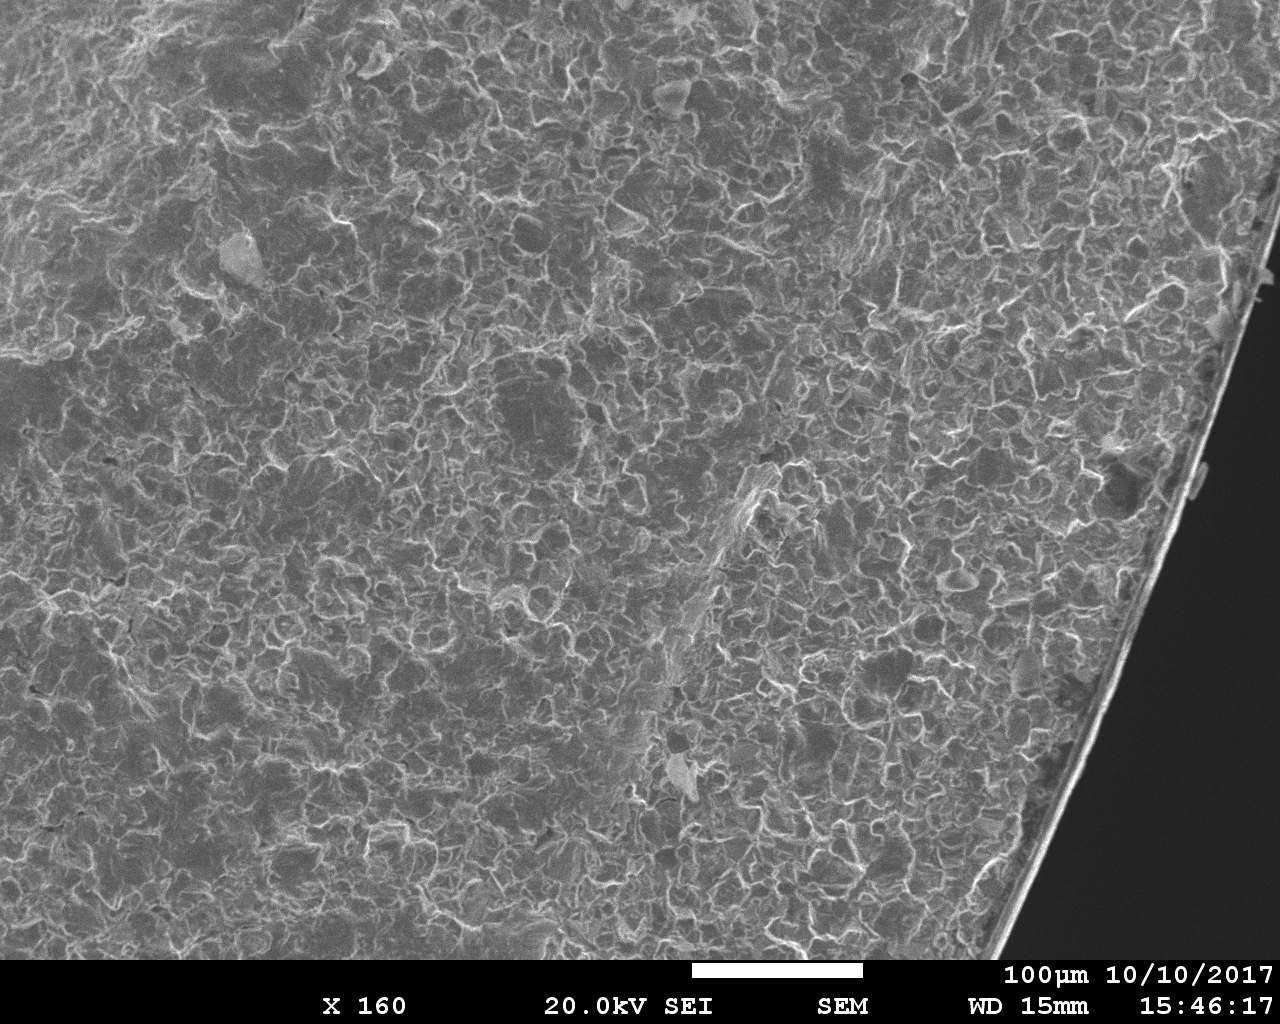
\includegraphics[width=6cm]{7206-1.jpg}
%     \centerline{(a)$\Delta \varepsilon_{eq}/2=0.55\%$.}
%   \end{minipage}%
%   \begin{minipage}[t]{0.5\linewidth}
%     \centering
%     \includegraphics[width=6cm]{7206-3.jpg}
%     \centerline{(b)$\Delta \varepsilon_{eq}/2=0.55\%$.}
%   \end{minipage}
%   \caption{TC-IP-TGMF.}
%   \label{Fig:MicrostructureofInconel718}
% \end{figure}

% \begin{figure}
%   \begin{minipage}[t]{0.5\linewidth}
%   \nonumber
%     \centering
%     \includegraphics[width=6cm]{720719.jpg}
%     \centerline{(a)$\Delta \varepsilon_{eq}/2=0.55\%$.}
%   \end{minipage}%
%   \begin{minipage}[t]{0.5\linewidth}
%     \centering
%     \includegraphics[width=6cm]{720721.jpg}
%     \centerline{(b)$\Delta \varepsilon_{eq}/2=0.55\%$.}
%   \end{minipage}

%   \begin{minipage}[t]{0.5\linewidth}
%   \nonumber
%     \centering
%     \includegraphics[width=6cm]{720932.jpg}
%     \centerline{(a)$\Delta \varepsilon_{eq}/2=0.45\%$.}
%   \end{minipage}%
%   \begin{minipage}[t]{0.5\linewidth}
%     \centering
%     \includegraphics[width=6cm]{720935.jpg}
%     \centerline{(b)$\Delta \varepsilon_{eq}/2=0.45\%$.}
%   \end{minipage}

%   \caption{TC-OP-TGMF.}
%   \label{Fig:MicrostructureofInconel718}
% \end{figure}

% \begin{figure}
%   \begin{minipage}[t]{0.5\linewidth}
%   \nonumber
%     \centering
%     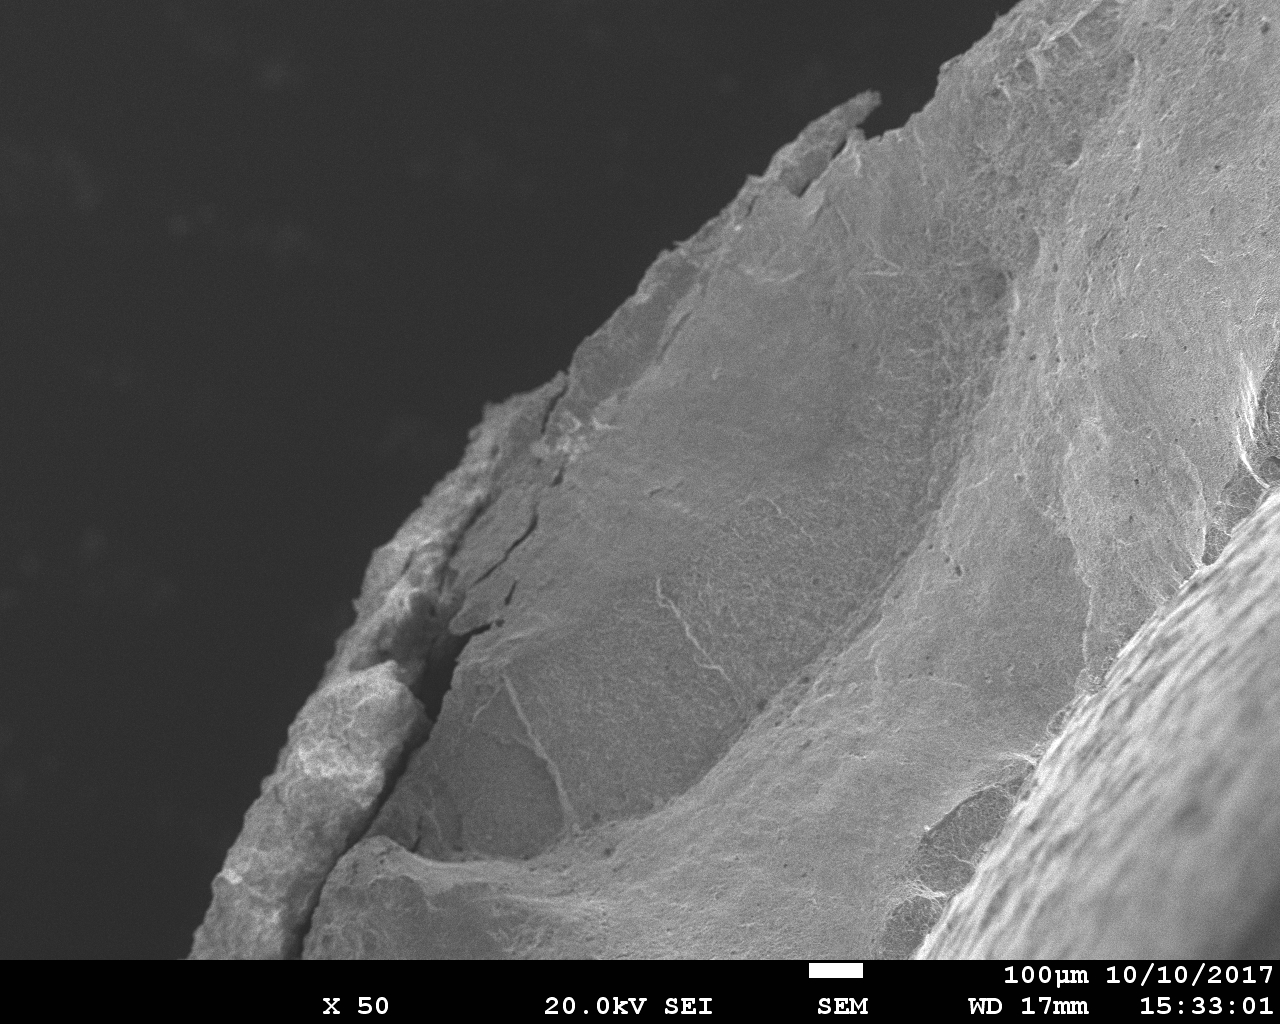
\includegraphics[width=6cm]{7301-7.jpg}
%     \centerline{(a)$\Delta \varepsilon_{eq}/2=0.55\%$.}
%   \end{minipage}%
%   \begin{minipage}[t]{0.5\linewidth}
%     \centering
%     \includegraphics[width=6cm]{7301-4.jpg}
%     \centerline{(b)$\Delta \varepsilon_{eq}/2=0.55\%$.}
%   \end{minipage}

%   \begin{minipage}[t]{0.5\linewidth}
%   \nonumber
%     \centering
%     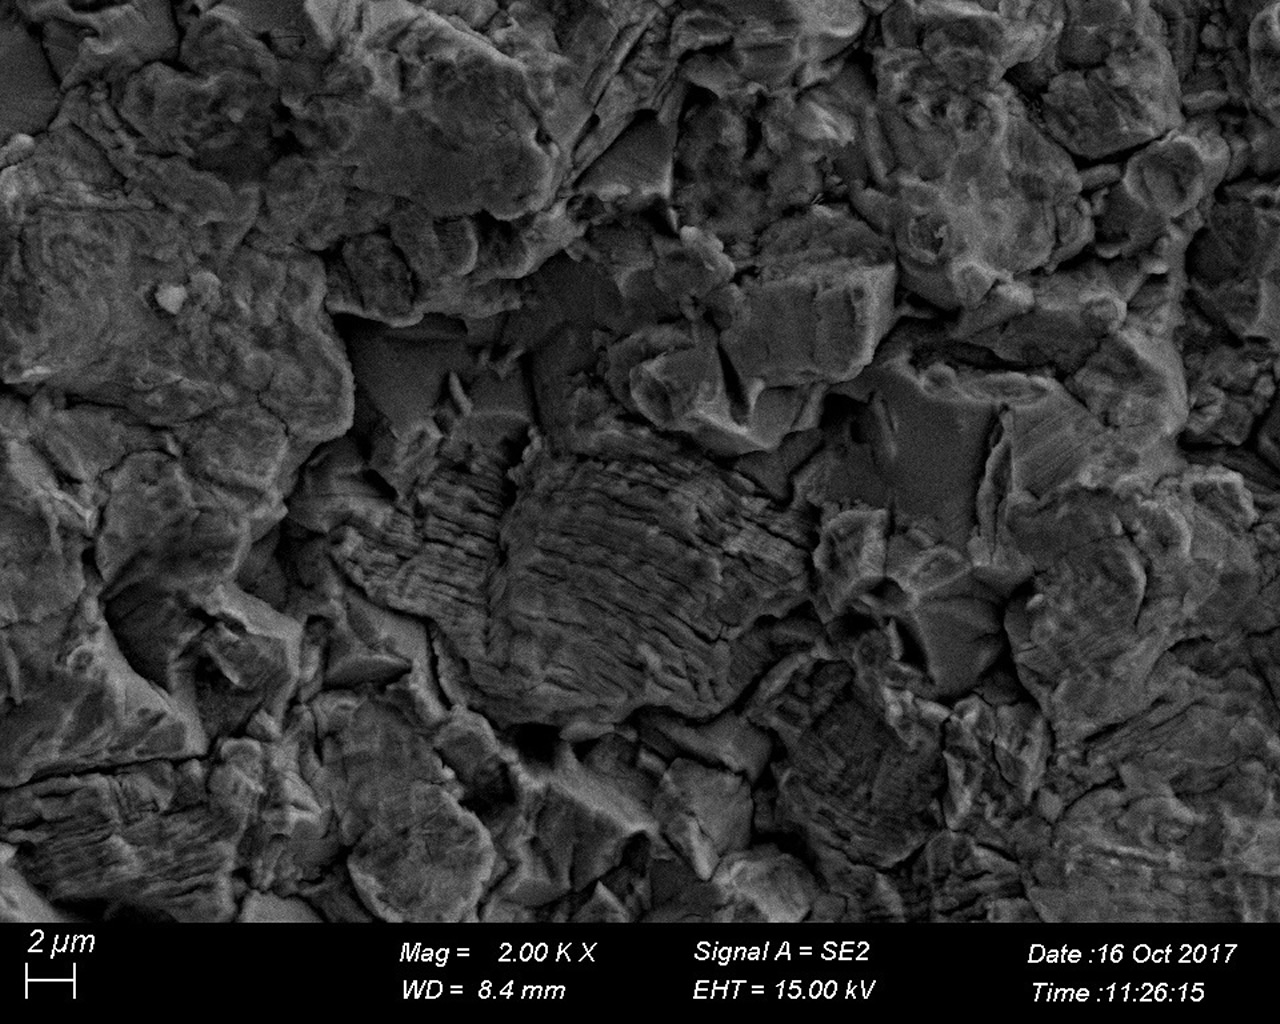
\includegraphics[width=6cm]{730109.jpg}
%     \centerline{(a)$\Delta \varepsilon_{eq}/2=0.55\%$.}
%   \end{minipage}%
%   \begin{minipage}[t]{0.5\linewidth}
%     \centering
%     \includegraphics[width=6cm]{730116.jpg}
%     \centerline{(b)$\Delta \varepsilon_{eq}/2=0.55\%$.}
%   \end{minipage}

%   \caption{TC-IP-TGMF-TBC.}
%   \label{Fig:MicrostructureofInconel718}
% \end{figure}

% \begin{figure}
%   \begin{minipage}[t]{0.5\linewidth}
%   \nonumber
%     \centering
%     \includegraphics[width=6cm]{7112-4.jpg}
%     \centerline{(a)TC-IF-650$^{\circ}$ $\Delta \varepsilon_{eq}/2=0.45\%$.}
%   \end{minipage}%
%   \begin{minipage}[t]{0.5\linewidth}
%     \centering
%     \includegraphics[width=6cm]{7047-7.jpg}
%     \centerline{(b)TC-IP $\Delta \varepsilon_{eq}/2=0.7\%$.}
%   \end{minipage}

%   \begin{minipage}[t]{0.5\linewidth}
%   \nonumber
%     \centering
%     \includegraphics[width=6cm]{7033-11.jpg}
%     \centerline{(c)TC-OP $\Delta \varepsilon_{eq}/2=0.65\%$.}
%   \end{minipage}%
%   \begin{minipage}[t]{0.5\linewidth}
%     \centering
%     \includegraphics[width=6cm]{7040-5.jpg}
%     \centerline{(d)PRO-IP $\Delta \varepsilon_{eq}/2=0.6\%$.}
%   \end{minipage}

%   \begin{minipage}[t]{0.5\linewidth}
%     \centering
%     \includegraphics[width=6cm]{7036-3.jpg}
%     \centerline{(e)NPR-IP $\Delta \varepsilon_{eq}/2=0.5\%$.}
%   \end{minipage}%
%   \begin{minipage}[t]{0.5\linewidth}
%     \centering
%     \includegraphics[width=6cm]{7046-8.jpg}
%     \centerline{(f)NPR-IP $\Delta \varepsilon_{eq}/2=0.7\%$.}
%   \end{minipage}
%   \caption{Observation of fatigue striations on fractures surface.}
%   \label{Fig:MicrostructureofInconel718}
% \end{figure}

% \begin{figure}
%   \begin{minipage}[t]{0.5\linewidth}
%   \nonumber
%     \centering
%     \includegraphics[width=6cm]{720935.jpg}
%     \centerline{(d)TC-OP-TGMF $\Delta \varepsilon_{eq}/2=0.50\%$.}
%   \end{minipage}%
%   \begin{minipage}[t]{0.5\linewidth}
%     \centering
%     \includegraphics[width=6cm]{720721.jpg}
%     \centerline{(c)TC-OP-TGMF $\Delta \varepsilon_{eq}/2=0.55\%$.}
%   \end{minipage}

%   \begin{minipage}[t]{0.5\linewidth}
%   \nonumber
%     \centering
%     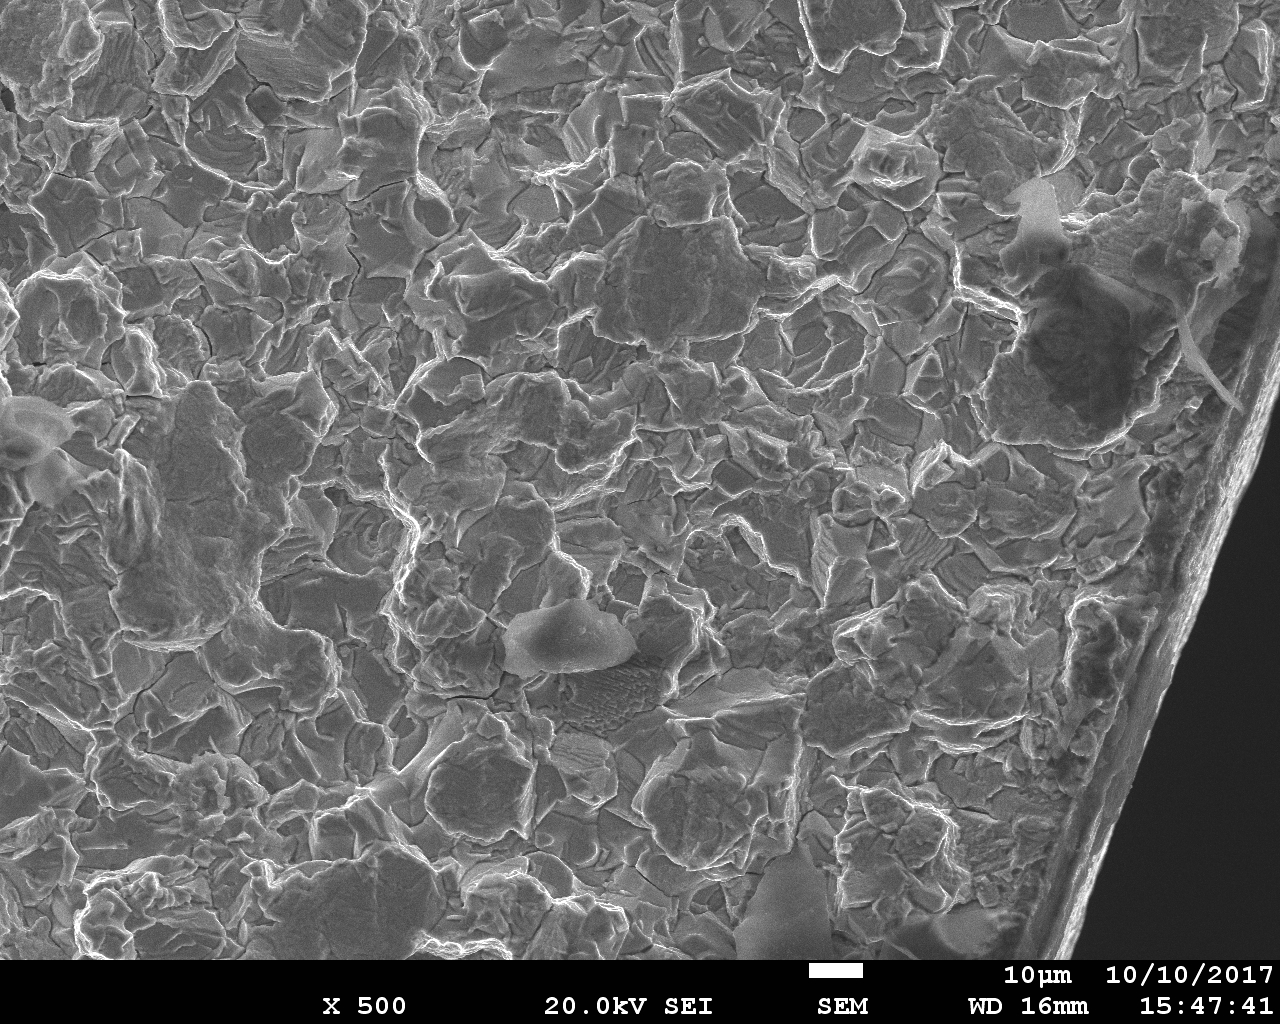
\includegraphics[width=6cm]{7206-2.jpg}
%     \centerline{(d)TC-IP-TGMF $\Delta \varepsilon_{eq}/2=0.55\%$.}
%   \end{minipage}%
%   \begin{minipage}[t]{0.5\linewidth}
%     \centering
%     \includegraphics[width=6cm]{730112.jpg}
%     \centerline{(c)TC-IP-TGMF-TBC $\Delta \varepsilon_{eq}/2=0.55\%$.}
%   \end{minipage}

%   \caption{Observation of fatigue striations on fractures surface.}
%   \label{Fig:MicrostructureofInconel718}
% \end{figure}

\section*{Acknowledgement:}

\bibliographystyle{unsrt}            % bibliography style
%\bibliographystyle{plain}            % bibliography style
\bibliography{bibliography}          % personal bibliography file

\end{document} 